\documentclass{article}

\usepackage[utf8]{inputenc}
\usepackage[T1]{fontenc}
\usepackage{lipsum}
\usepackage{graphicx}
\usepackage{amsmath}
\usepackage[margin=1in]{geometry}
\usepackage{titlesec}
\usepackage{enumitem}
\usepackage{geometry}
\usepackage{tabularx}
\usepackage{caption}
\usepackage{fixltx2e}
\usepackage{booktabs}
\usepackage{float}  
\usepackage{graphicx}
\usepackage{floatflt,epsfig}
\usepackage[margin=1in]{geometry} 
\usepackage{lipsum}
\usepackage{graphicx}
\usepackage{listings}
\usepackage{xcolor}
\usepackage{color}

\lstdefinelanguage{Java}{
  keywords={abstract,assert,boolean,break,byte,case,catch,char,class,const,continue,default,do,double,else,enum,extends,false,final,finally,float,for,goto,if,implements,import,instanceof,int,interface,long,native,new,null,package,private,protected,public,return,short,static,strictfp,super,switch,synchronized,this,throw,throws,transient,true,try,void,volatile,while},
  morekeywords={[2]System,out},
  morecomment=[l]{//},
  morecomment=[s]{/*}{*/},
  morestring=[b]",
  basicstyle=\small\ttfamily,
  keywordstyle=\color{blue}\bfseries,
  keywordstyle={[2]\color{orange}\bfseries},
  commentstyle=\color{green!70!black},
  stringstyle=\color{red},
  showstringspaces=false,
  tabsize=2,
  breaklines=true,
  breakatwhitespace=true,
  frame=single, 
  captionpos=b
}

\titleformat{\section}[block]
{\large\bfseries}{\thesection}{1em}{}

\titleformat{\subsection}[block]
{\normalfont\large\bfseries}{\thesubsection}{1em}{}

\begin{document}

\pagestyle{empty}

\begin{titlepage} 
\begin{center}
    {{\Large{\textsc{Alma Mater Studiorum - Università di Bologna}}}}
    \rule[0.1cm]{\textwidth}{0.1px}
    \rule[0.5cm]{\textwidth}{0.6px}\\
    {\large{SCUOLA DI SCIENZE \\ Corso di Laurea in Informatica per il Management}}
\end{center}

\vspace{50px}

\begin{center}
    {\LARGE{{\bf storJ}}}\
\end{center}

\vspace{115px}
\par
\noindent
\begin{minipage}[t]{0.04\textwidth}
~
\end{minipage}
\begin{minipage}[t]{0.4\textwidth}
\end{minipage}
\hfill
\begin{minipage}[t]{0.4\textwidth}\raggedleft
    {\fontsize{12}{13}{DOCUMENTAZIONE SVOLTA DA:}\
\fontsize{12}{13}{\it Canghiari Matteo, 1032059 \ De Rosa Davide, 1054948 \ Ghazanfar Tabish, 1045078 \ Nadifi Ossama, 1021258}}
\end{minipage}
\begin{minipage}[t]{0.04\textwidth}
~
\end{minipage}

\vspace*{210px}

\begin{center}
    \large{Anno Accademico 2023/2024}
\end{center}
\end{titlepage}

\section{Design Model}

\subsection{Modello di dominio} 
\large

\subsection{Diagramma dei casi d'uso}
\large
\begin{center}
    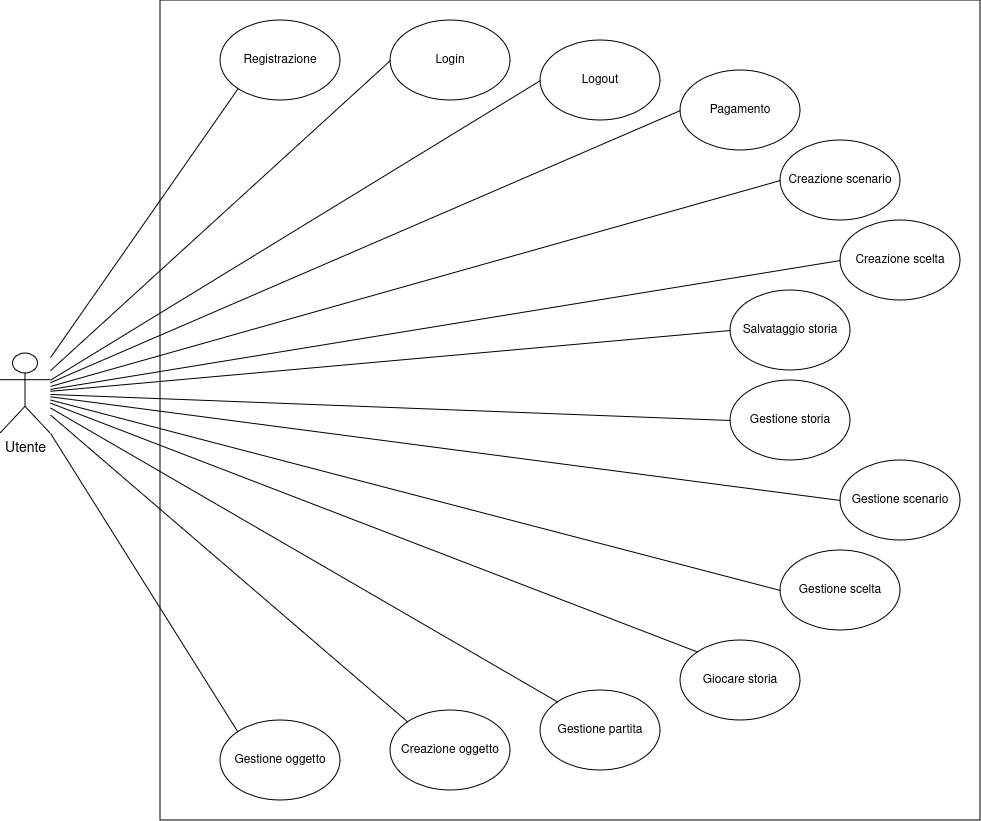
\includegraphics[width=0.7\textwidth]{foto2.png}
\end{center}

\newpage
\textbf{Registrazione}
\begin{itemize}[label = { }]
    \itemsep0px
    \item ID: UC1 - Registrazione
    \item Attori: Utente
    \item Precondizioni: 
        \begin{itemize}[label = {-}]
            \item Non presente
        \end{itemize}
    \item Main sequence: 
        \begin{enumerate}
            \item Utente inserisce e invia i dati
            \item Sistema acquisisce e salva i dati
            \item Sistema invia esito positivo
            \item Utente visualizza esito positivo
        \end{enumerate}
    \item Alternative sequence:
        \begin{enumerate}
            \item Utente inserisce e invia i dati non idonei
            \item Sistema acquisisce e individua un errore
            \item Sistema invia esito negativo
            \item Utente visualizza esito negativo
        \end{enumerate}
    \item Postcondizioni: 
        \begin{itemize}[label = {-}]
            \item Sistema salva i dati nella piattaforma
        \end{itemize}
\end{itemize}
\textbf{Login}
\begin{itemize}[label = { }]
    \itemsep0px
    \item ID: UC2 - Login
    \item Attori: Utente
    \item Precondizioni: 
        \begin{itemize}[label = {-}]
            \item Utente ha effettuato la registrazione
        \end{itemize}
    \item Main sequence: 
        \begin{enumerate}
            \item Utente inserisce e invia i dati
            \item Sistema acquisisce e confronta con i dati salvati
            \item Sistema nega l'accesso e invia esito positivo
            \item Utente visualizza esito positivo
        \end{enumerate}
    \item Alternative sequence:
        \begin{enumerate}
            \item Utente inserisce e invia i dati non idonei
            \item Sistema acquisisce e individua un errore
            \item Sistema invia esito negativo
            \item Utente visualizza esito negativo
        \end{enumerate}
    \item Postcondizioni: 
        \begin{itemize}[label = {-}]
            \item Utente autenticato dalla piatttaforma
        \end{itemize}
\end{itemize}
\textbf{Logout}
\begin{itemize}[label = { }]
    \itemsep0px
    \item ID: UC3 - Logout
    \item Attori: Utente
    \item Precondizioni: 
        \begin{itemize}[label = {-}]
            \item Utente autenticato dalla piattaforma
        \end{itemize}
    \item Main sequence: 
        \begin{enumerate}
            \item Utente effettua la selezione di logout
            \item Sistema registra lo stato Utente
        \end{enumerate}
    \item Alternative sequence:
        \begin{enumerate}
            \item Non presente
        \end{enumerate}
    \item Postcondizioni: 
        \begin{itemize}[label = {-}]
            \item Utente disconesso dalla piatttaforma
        \end{itemize}
\end{itemize}
\textbf{Pagamento}
\begin{itemize}[label = { }]
    \itemsep0px
    \item ID: UC4 - Pagamento
    \item Attori: Utente
    \item Precondizioni: 
        \begin{itemize}[label = {-}]
            \item Utente autenticato dalla piattaforma
            \item Utente non abbia effettuato alcun pagamento
        \end{itemize}
    \item Main sequence: 
        \begin{enumerate}
            \item Utente inserisce e invia i dati
            \item Sistema acquisisce i dati
            \item Sistema processa pagamento e invia esito positivo
            \item Utente visualizza esito positivo
        \end{enumerate}
    \item Alternative sequence:
        \begin{enumerate}
            \item Utente inserisce e invia i dati
            \item Sistema acquisisce i dati
            \item Sistema processa pagamento e invia esito negativo
            \item Utente visualizza esito negativo
        \end{enumerate}
    \item Postcondizioni: 
        \begin{itemize}[label = {-}]
            \item Sistema salva lo stato Utente di pagamento
        \end{itemize}
\end{itemize}
\textbf{Creazione scenario}
\begin{itemize}[label = { }]
    \itemsep0px
    \item ID: UC5 - Creazione scenario
    \item Attori: Utente
    \item Precondizioni: 
        \begin{itemize}[label = {-}]
            \item Utente autenticato dalla piattaforma
        \end{itemize}
    \item Main sequence: 
        \begin{enumerate}
            \item Utente inserisce e invia i dati
            \item Sistema acquisisce i dati
            \item Sistema controlla i dati e invia esito positivo
            \item Utente visualizza esito positivo
        \end{enumerate}
    \item Alternative sequence:
        \begin{enumerate}
            \item Utente inserisce e invia i dati non completi
            \item Sistema acquisisce i dati
            \item Sistema controlla i dati e invia esito negativo
            \item Utente visualizza esito negativo
        \end{enumerate}
    \item Postcondizioni: 
        \begin{itemize}[label = {-}]
            \item Sistema salva i dati Scenario
        \end{itemize}
\end{itemize}
\textbf{Creazione scelta}
\begin{itemize}[label = { }]
    \itemsep0px
    \item ID: UC6 - Creazione scelta
    \item Attori: Utente
    \item Precondizioni: 
        \begin{itemize}[label = {-}]
            \item Utente autenticato dalla piattaforma
            \item Utente abbia creato componenti Scenario
        \end{itemize}
    \item Main sequence: 
        \begin{enumerate}
            \item Utente inserisce e invia i dati
            \item Sistema acquisisce i dati
            \item Sistema controlla i dati e invia esito positivo
            \item Utente visualizza esito positivo
        \end{enumerate}
    \item Alternative sequence:
        \begin{enumerate}
            \item Utente inserisce e invia i dati non completi
            \item Sistema acquisisce i dati
            \item Sistema controlla i dati e invia esito negativo
            \item Utente visualizza esito negativo
        \end{enumerate}
    \item Postcondizioni: 
        \begin{itemize}[label = {-}]
            \item Sistema salva i dati Scelta
        \end{itemize}
\end{itemize}
\textbf{Salvataggio storia}
\begin{itemize}[label = { }]
    \itemsep0px
    \item ID: UC7 - Salvataggio storia
    \item Attori: Utente
    \item Precondizioni: 
        \begin{itemize}[label = {-}]
            \item Utente autenticato dalla piattaforma
            \item Utente abbia creato componenti Scenario
            \item Utente abbia creato componenti Scelta
        \end{itemize}
    \item Main sequence: 
        \begin{enumerate}
            \item Utente richiede salvataggio Storia
            \item Sistema acquisisce i dati
            \item Sistema controlla i parametri di salvataggio
            \item Sistema invia esito positivo
            \item Utente visualizza esito positivo
        \end{enumerate}
    \item Alternative sequence:
        \begin{enumerate}
            \item Utente richiede salvataggio Storia
            \item Sistema acquisisce i dati
            \item Sistema controlla i parametri di salvataggio
            \item Sistema invia esito negativo
            \item Utente visualizza esito negativo
        \end{enumerate}
    \item Postcondizioni: 
        \begin{itemize}[label = {-}]
            \item Sistema salva i dati Storia
            \item Sistema rende componente Storia giocabile
        \end{itemize}
\end{itemize}
\textbf{Gestione storia}
\begin{itemize}[label = { }]
    \itemsep0px
    \item ID: UC8 - Gestione storia
    \item Attori: Utente
    \item Precondizioni: 
        \begin{itemize}[label = {-}]
            \item Utente autenticato dalla piattaforma
        \end{itemize}
    \item Main sequence: 
        \begin{enumerate}
            \item Utente richiede rimozione della Storia
            \item Sistema riceve richiesta
        \end{enumerate}
    \item Alternative sequence:
        \begin{enumerate}
            \item Non presente
        \end{enumerate}
    \item Postcondizioni: 
        \begin{itemize}[label = {-}]
            \item Sistema elimina componente Storia
        \end{itemize}
\end{itemize}
\textbf{Gestione scenario}
\begin{itemize}[label = { }]
    \itemsep0px
    \item ID: UC9 - Gestione scenario
    \item Attori: Utente
    \item Precondizioni: 
        \begin{itemize}[label = {-}]
            \item Utente autenticato dalla piattaforma
        \end{itemize}
    \item Main sequence: 
        \begin{enumerate}
            \item Utente richiede rimozione dello Scenario
            \item Sistema riceve richiesta
        \end{enumerate}
    \item Alternative sequence:
        \begin{enumerate}
            \item Utente richiede modifica testuale dello Scenario
            \item Sistema riceve richiesta
            \item Utente inserisci i dati sostitutivi
            \item Sistema acquisisce modifiche
        \end{enumerate}
    \item Postcondizioni: 
        \begin{itemize}[label = {-}]
            \item Sistema elimina componente Scenario
            \item Sistema modifica Scenario
        \end{itemize}
\end{itemize}
\textbf{Gestione scelta}
\begin{itemize}[label = { }]
    \itemsep0px
    \item ID: UC10 - Gestione scelta
    \item Attori: Utente
    \item Precondizioni: 
        \begin{itemize}[label = {-}]
            \item Utente autenticato dalla piattaforma
        \end{itemize}
    \item Main sequence: 
        \begin{enumerate}
            \item Utente richiede rimozione della Scelta
            \item Sistema riceve richiesta
        \end{enumerate}
    \item Alternative sequence:
        \begin{enumerate}
            \item Utente richiede modifica testuale della Scelta
            \item Sistema riceve richiesta
            \item Utente inserisci i dati sostitutivi
            \item Sistema acquisisce modifiche
        \end{enumerate}
    \item Postcondizioni: 
        \begin{itemize}[label = {-}]
            \item Sistema elimina componente Scelta
            \item Sistema modifica Scelta
        \end{itemize}
\end{itemize}
\textbf{Gestione storia}
\begin{itemize}[label = { }]
    \itemsep0px
    \item ID: UC11 - Gestione storia
    \item Attori: Utente
    \item Precondizioni: 
        \begin{itemize}[label = {-}]
            \item Utente autenticato dalla piattaforma
            \item Utente abbia effettuato un pagamento
            \item Storia deve essere giocabile
        \end{itemize}
    \item Main sequence: 
        \begin{enumerate}
            \item Utente seleziona una Storia giocabile
            \item Sistema mostra Scenario composto dalle sue Scelte
            \item Utente indica Scelta
            \item Sistema acquisisce la Scelta
            \item Sistema mostra Scenario successivo
        \end{enumerate}
    \item Alternative sequence:
        \begin{enumerate}
            \item Utente seleziona una Storia giocabile
            \item Sistema mostra Scenario composto dalle sue Scelte
            \item Utente indica Scelta
            \item Sistema acquisisce la Scelta
            \item Sistema mostra Scenario finale
        \end{enumerate}
    \item Postcondizioni: 
        \begin{itemize}[label = {-}]
            \item Sistema salva la Partita
        \end{itemize}
\end{itemize}
\textbf{Gestione partita}
\begin{itemize}[label = { }]
    \itemsep0px
    \item ID: UC12 - Gestione partita
    \item Attori: Utente
    \item Precondizioni: 
        \begin{itemize}[label = {-}]
            \item Utente autenticato dalla piattaforma
            \item Utente abbia effettuato un pagamento
            \item Storia deve essere giocabile
        \end{itemize}
    \item Main sequence: 
        \begin{enumerate}
            \item Utente richiede rimozione Partita inerente alla Storia
            \item Sistema riceve richiesta
        \end{enumerate}
    \item Alternative sequence:
        \begin{enumerate}
            \item Utente seleziona una Partita da riprendere
            \item Sistema mostra Scenario composto dalle sue Scelte
            \item Utente indica Scelta
            \item Sistema acquisisce la Scelta
            \item Sistema mostra Scenario Successivo
        \end{enumerate}
    \item Postcondizioni: 
        \begin{itemize}[label = {-}]
            \item Sistema rimuove la Partita
            \item Utente riprende la Partita
        \end{itemize}
\end{itemize}
\textbf{Creazione oggetto}
\begin{itemize}[label = {-}]
    \itemsep0px
    \item ID: UC13 - Creazione oggetto
    \item Attori: Utente
    \item Precondizioni: 
        \begin{itemize}[label = {-}]
            \item Utente autenticato dalla piattaforma
        \end{itemize}
    \item Main sequence: 
        \begin{enumerate}
            \item Utente inserisce e invia i dati
            \item Sistema acquisisce i dati
            \item Sistema controlla i dati e invia esito positivo
            \item Utente visualizza esito positivo
        \end{enumerate}
    \item Alternative sequence:
        \begin{enumerate}
            \item Utente inserisce e invia i dati non completi
            \item Sistema acquisisce i dati
            \item Sistema controlla i dati e invia esito negativo
            \item Utente visualizza esito negativo
        \end{enumerate}
    \item Postcondizioni: 
        \begin{itemize}[label = {-}]
            \item Sistema salva i dati dell'Oggetto
        \end{itemize}
\end{itemize}
\textbf{Gestione oggetto}
\begin{itemize}[label = {-}]
    \itemsep0px
    \item ID: UC14 - Gestione oggetto
    \item Attori: Utente
    \item Precondizioni: 
        \begin{itemize}[label = {-}]
            \item Utente autenticato dalla piattaforma
        \end{itemize}
    \item Main sequence: 
        \begin{enumerate}
            \item Utente richiede rimozione dell'Oggetto
            \item Sistema riceve richiesta
        \end{enumerate}
    \item Alternative sequence:
        \begin{enumerate}
            \item Utente richiede modifica testuale dell'Oggetto
            \item Sistema riceve richiesta
            \item Utente inserisce modifiche
            \item Sistema acquisisce modifiche
        \end{enumerate}
    \item Postcondizioni: 
        \begin{itemize}[label = {-}]
            \item Sistema rimuove componente Oggetto
            \item Sistema modifica componente Oggetto
        \end{itemize}
\end{itemize}

\newpage
\subsection{Burndown chart}
\begin{center}
    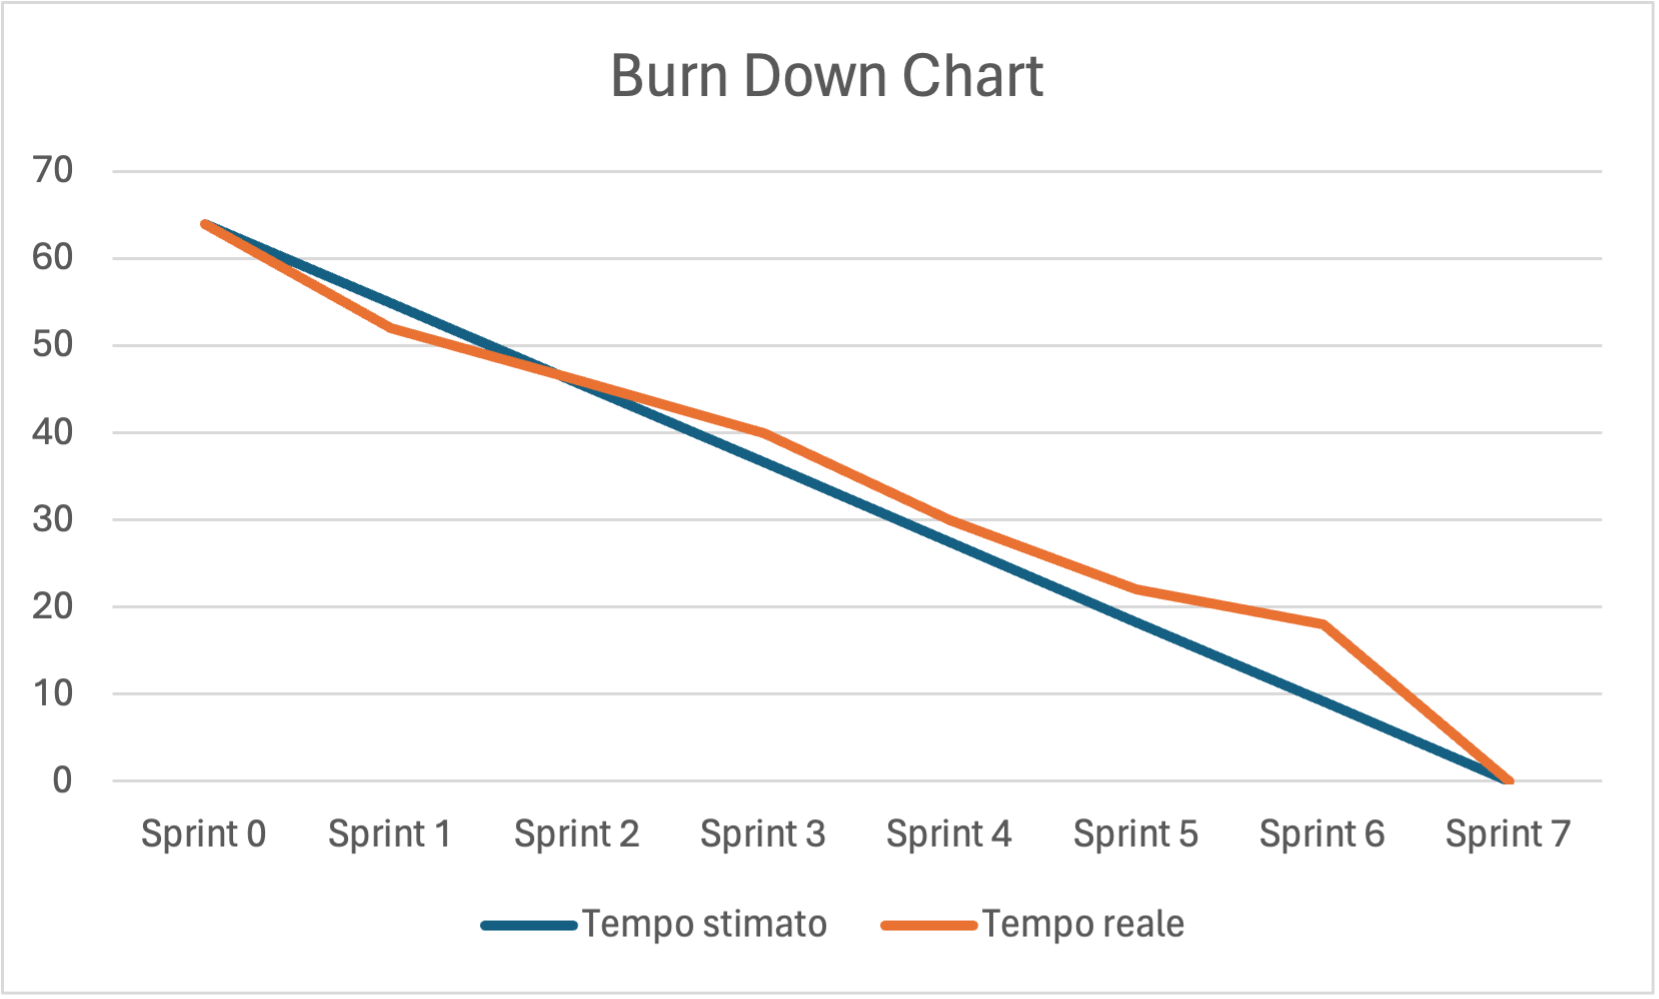
\includegraphics[width=0.7\textwidth]{foto3.png}
\end{center}

\newpage
\section{Manuale dell'utente}
\subsection*{Home}
Sezione a cui si accede avviando l'applicativo. All'interno di questa è possibile ottenere una breve descrizione del progetto, visualizzare le specifiche e la repository GitHub, ed infine accedere alla relazione. Dalla navbar si può accedere alle schermate di \textit{Accedi} e \textit{Registrati}.
\begin{center}
    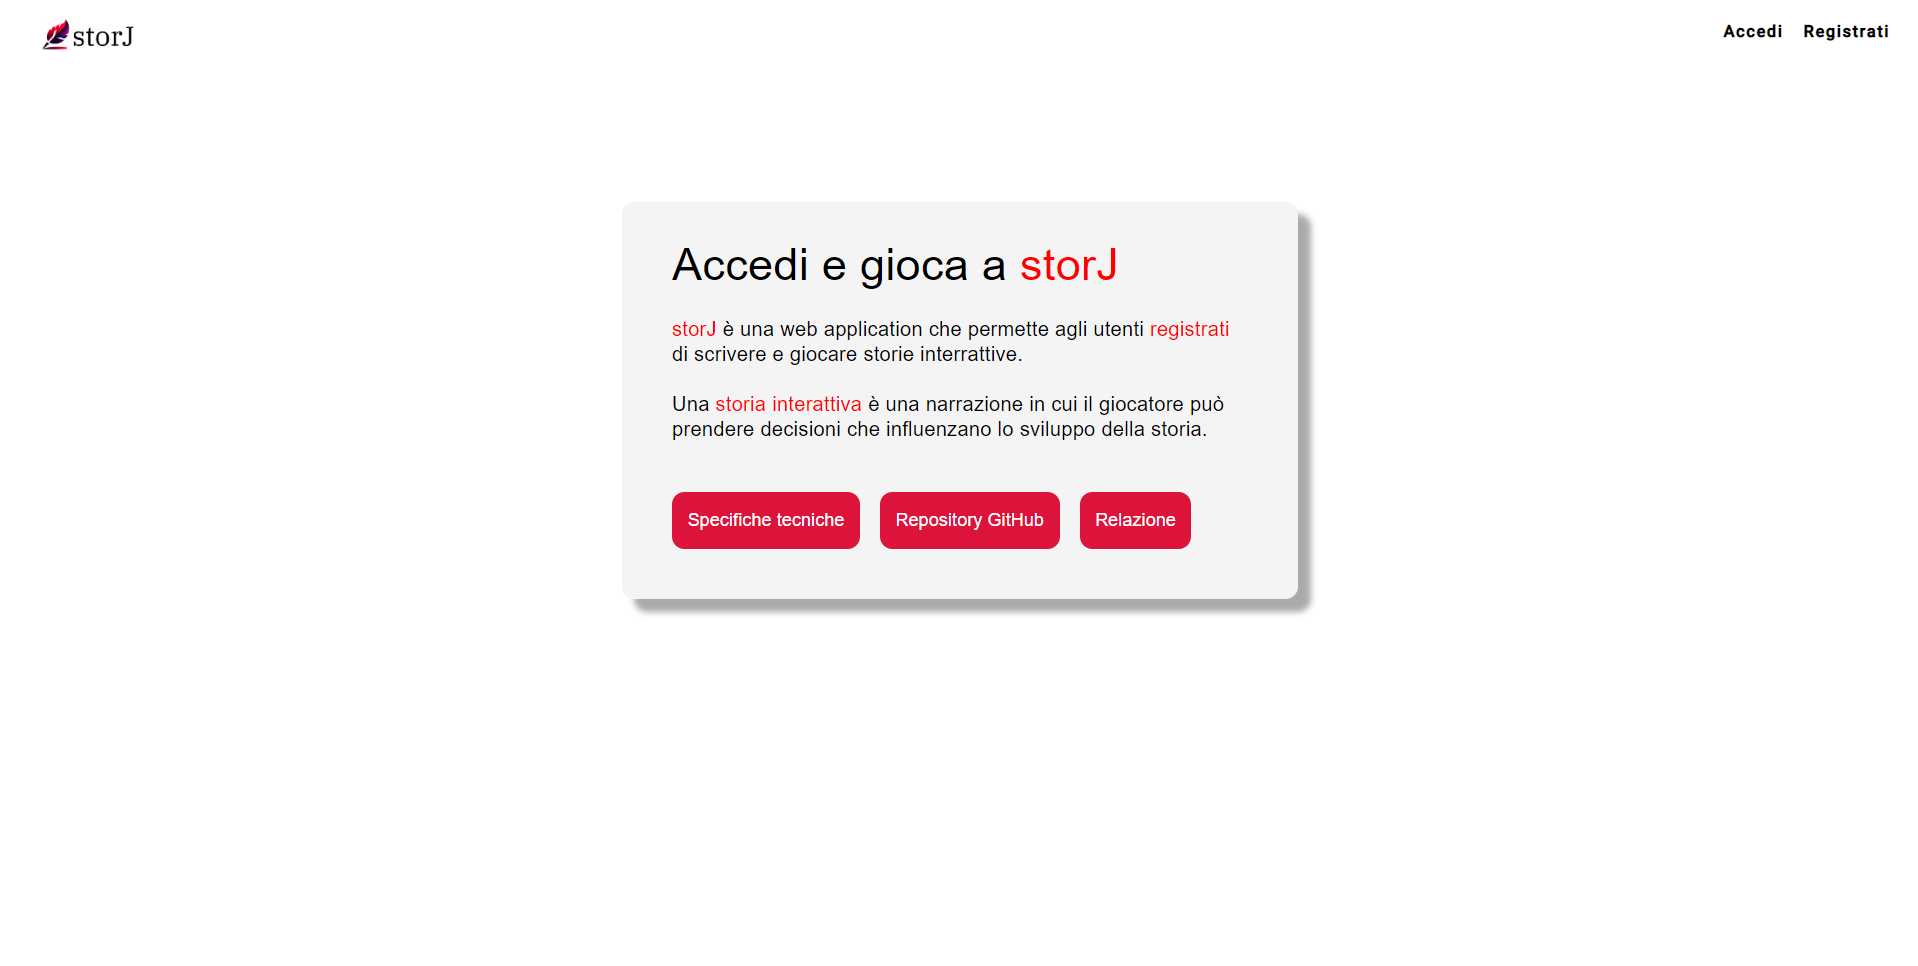
\includegraphics[width=0.8\textwidth]{foto4.png}
\end{center}

\subsection*{Registrazione}
Sezione che permette di registrarsi alla piattaforma. Offre la possibilità di accedere alla schermata di \textit{Accedi} sia tramite la schermata principale che tramite navbar.
\begin{center}
    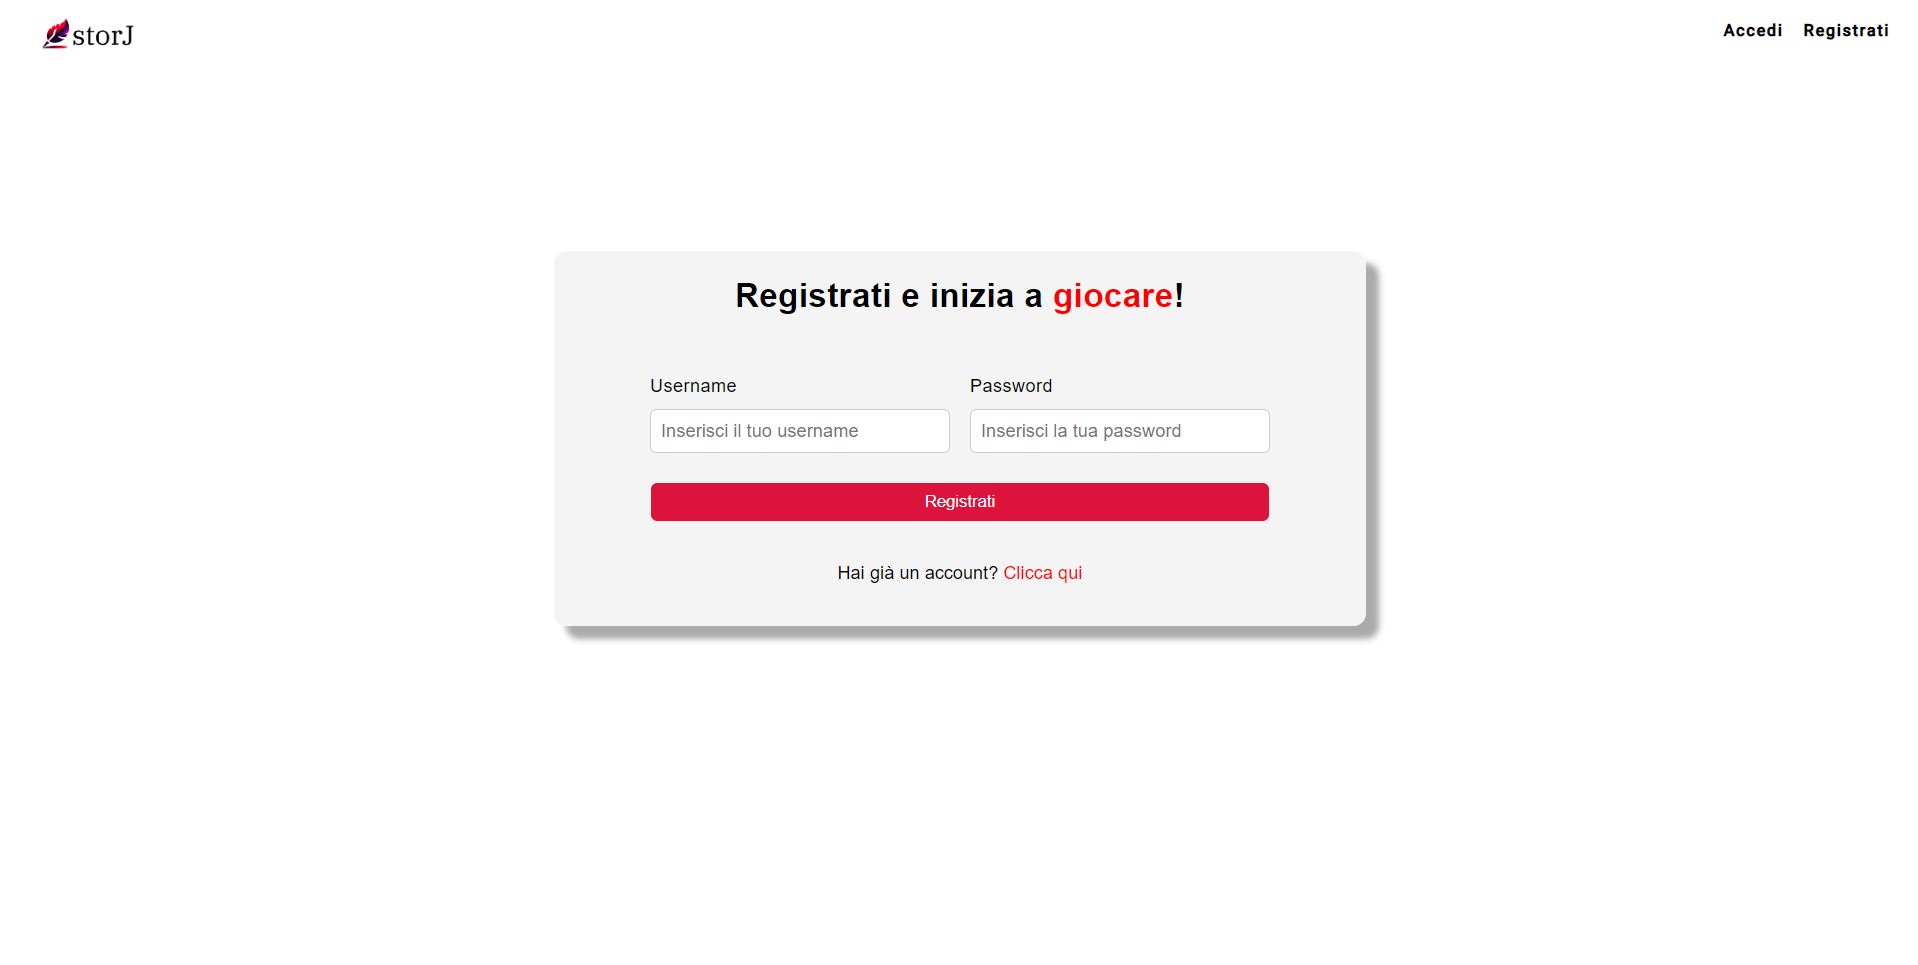
\includegraphics[width=0.8\textwidth]{foto5.png}
\end{center}

\subsection*{Accedi}
Sezione che permette di autenticarsi alla piattaforma. Offre la possibilità di accedere alla schermata di \textit{Registrazione} sia tramite la schermata principale che tramite navbar.
\begin{center}
    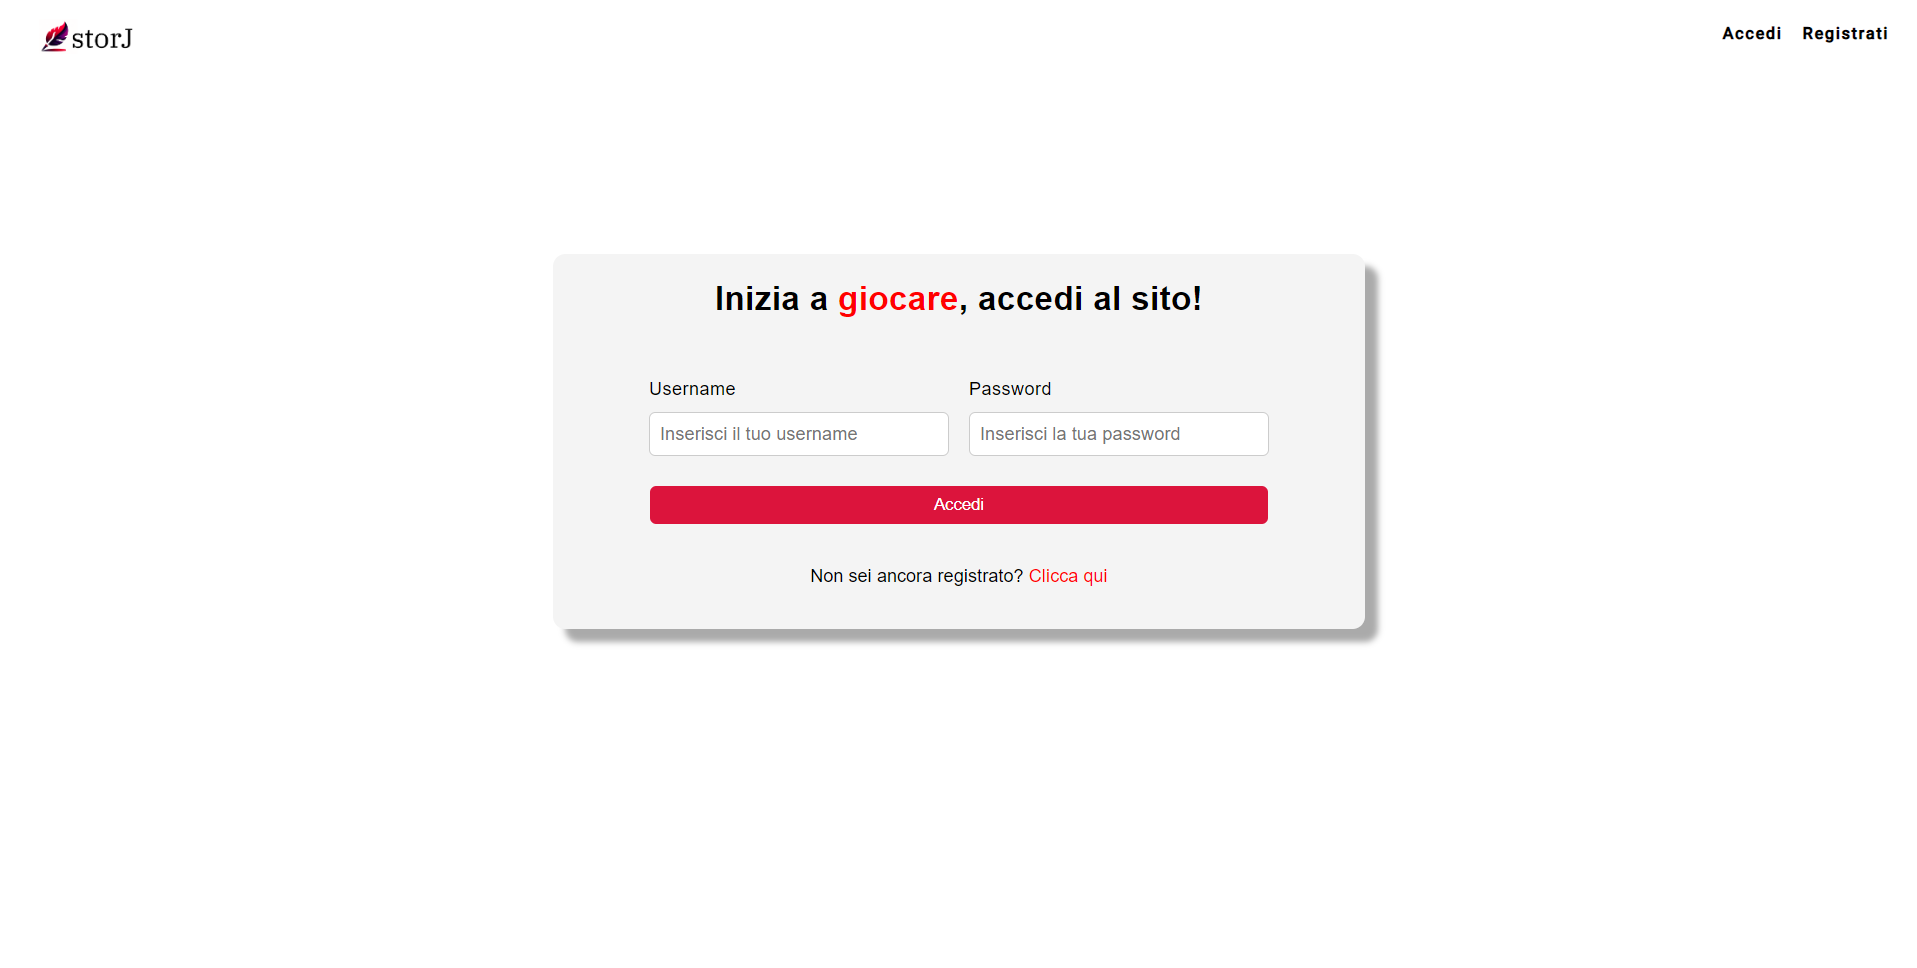
\includegraphics[width=0.8\textwidth]{foto6.png}
\end{center}

\subsection*{Homepage storJ}
Sezione a cui si accede in seguito all'autenticazione. Permette di visualizzare una breve descrizione delle azioni eseguibili. Attraverso la navbar si potranno raggiungere le schermate relative a \textit{Paga}, \textit{Crea}, ed infine effettuare il \textit{Logout}.
\begin{center}
    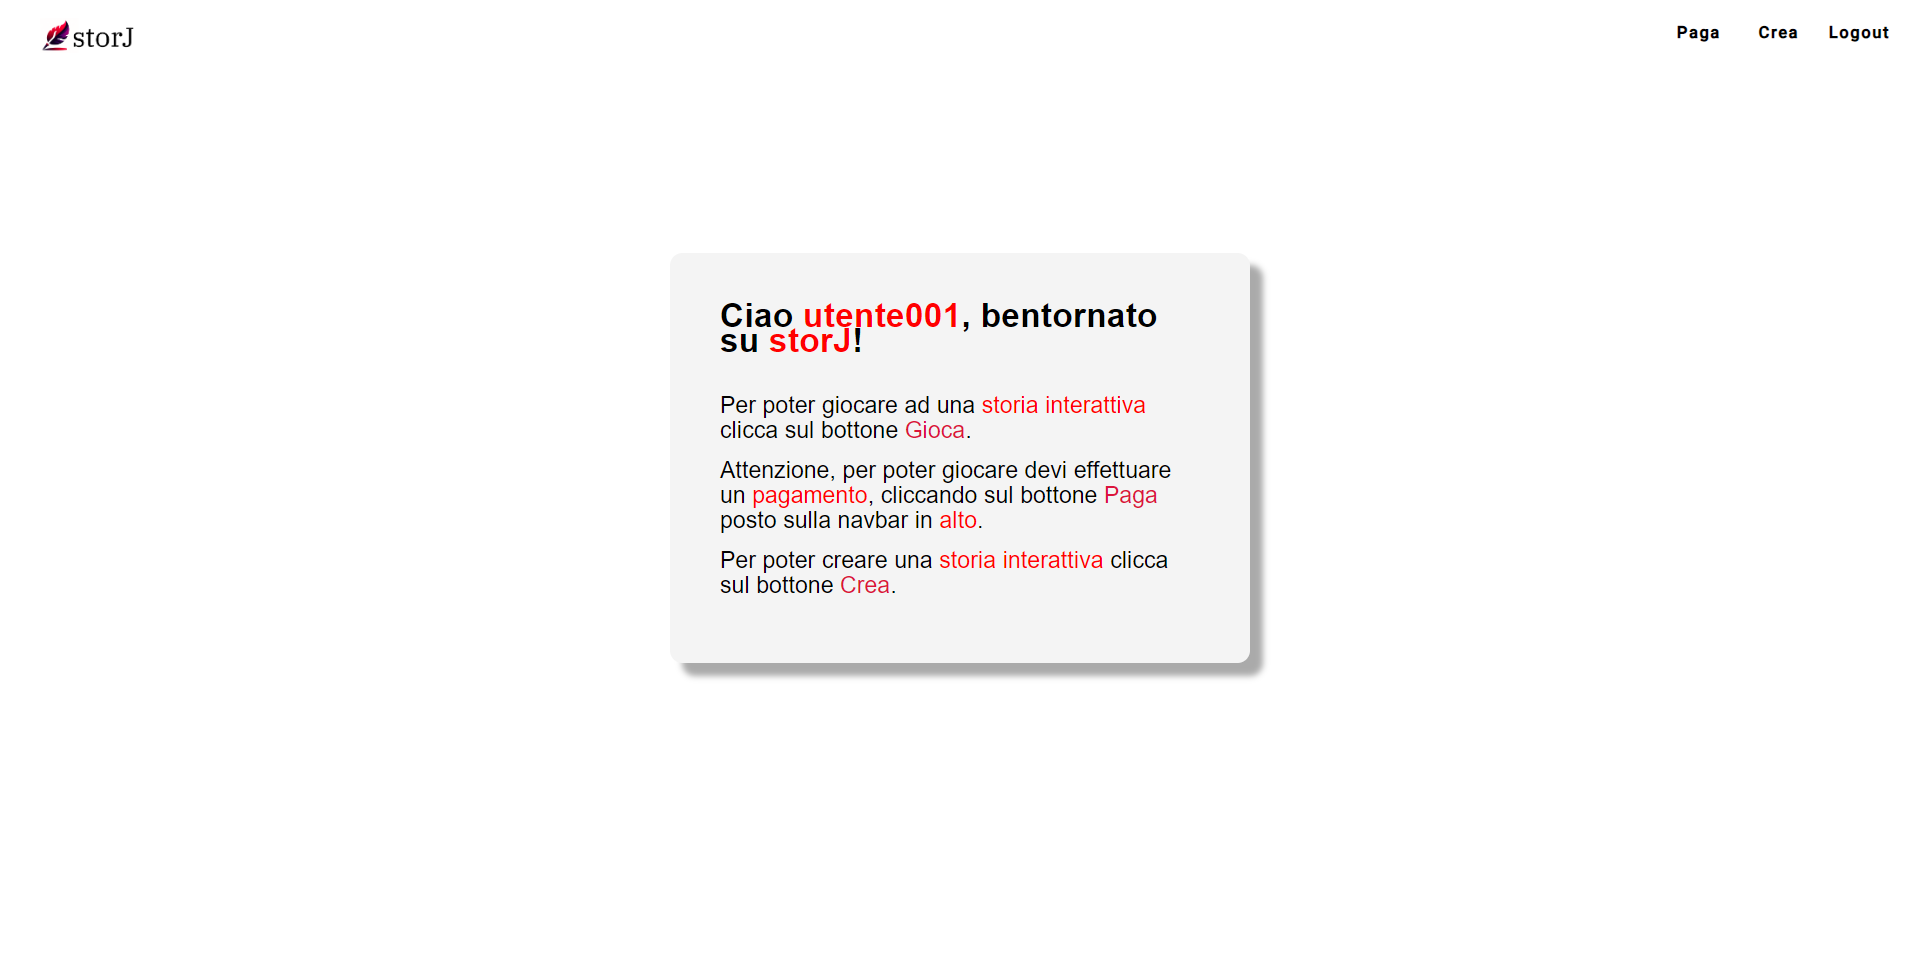
\includegraphics[width=0.8\textwidth]{foto7.png}
\end{center}
Nel caso in cui pagamento sia già stato effettuato, la voce \textit{Paga} sarà sostituita da \textit{Gioca}.

\subsection*{Paga}
Sezione che permette di effettuare il pagamento, in modo da poter sbloccare tutte le funzionalità della piattaforma. Sarà necessario inserire l'ammontare del pagamento, titolare e numero della carta, ed infine il relativo CVV. Potrebbe essere necessario effettuare più tentativi per far sì che vada a buon fine.
\begin{center}
    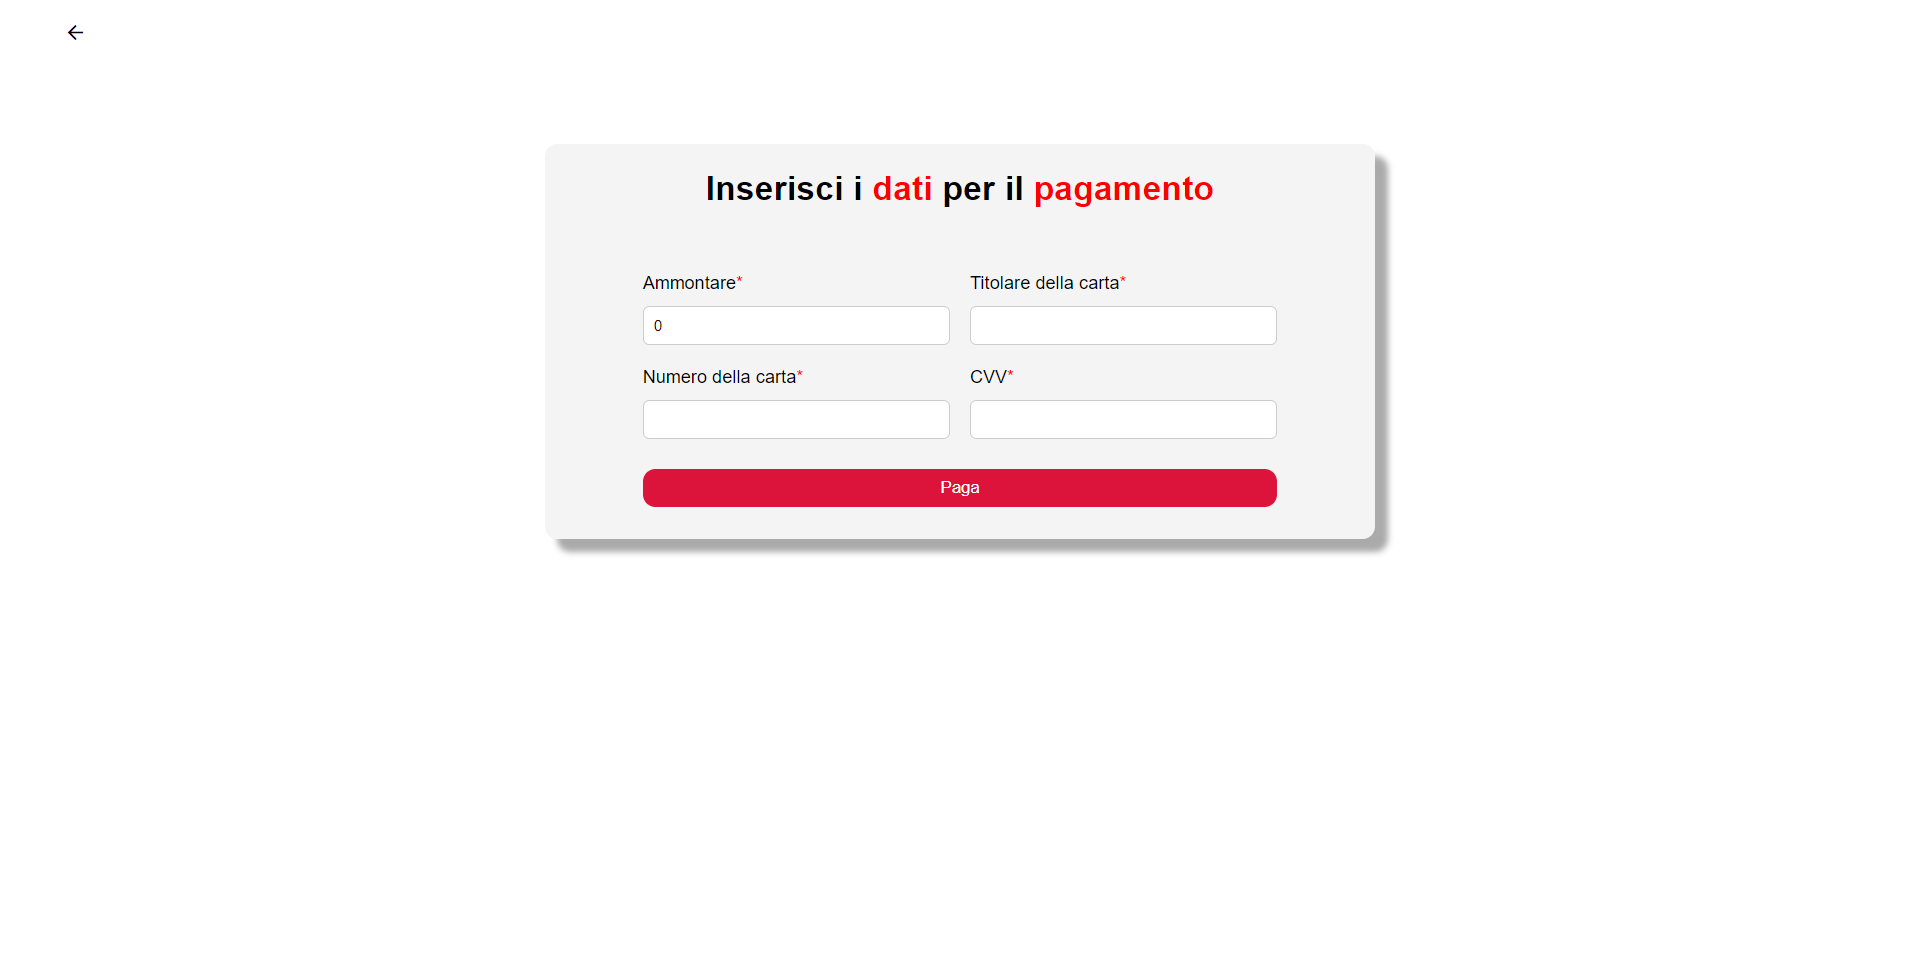
\includegraphics[width=0.8\textwidth]{foto8.png}
\end{center}

\subsection*{Storie}
Sezione che consente la gestione delle storie. Permette di visualizzare le storie create in precedenza. Ad ognuna di esse sono assegnati due bottoni, necessari per la \textit{modifica} e l'\textit{eliminazione}. È presente una navbar contenente il collegamento alla schermata dedicata alla \textit{creazione} delle storie. Nel caso la storia sia stata salvata, la \textit{modifica} permetterà solo di cambiare i testi all'interno di questa.
\begin{center}
    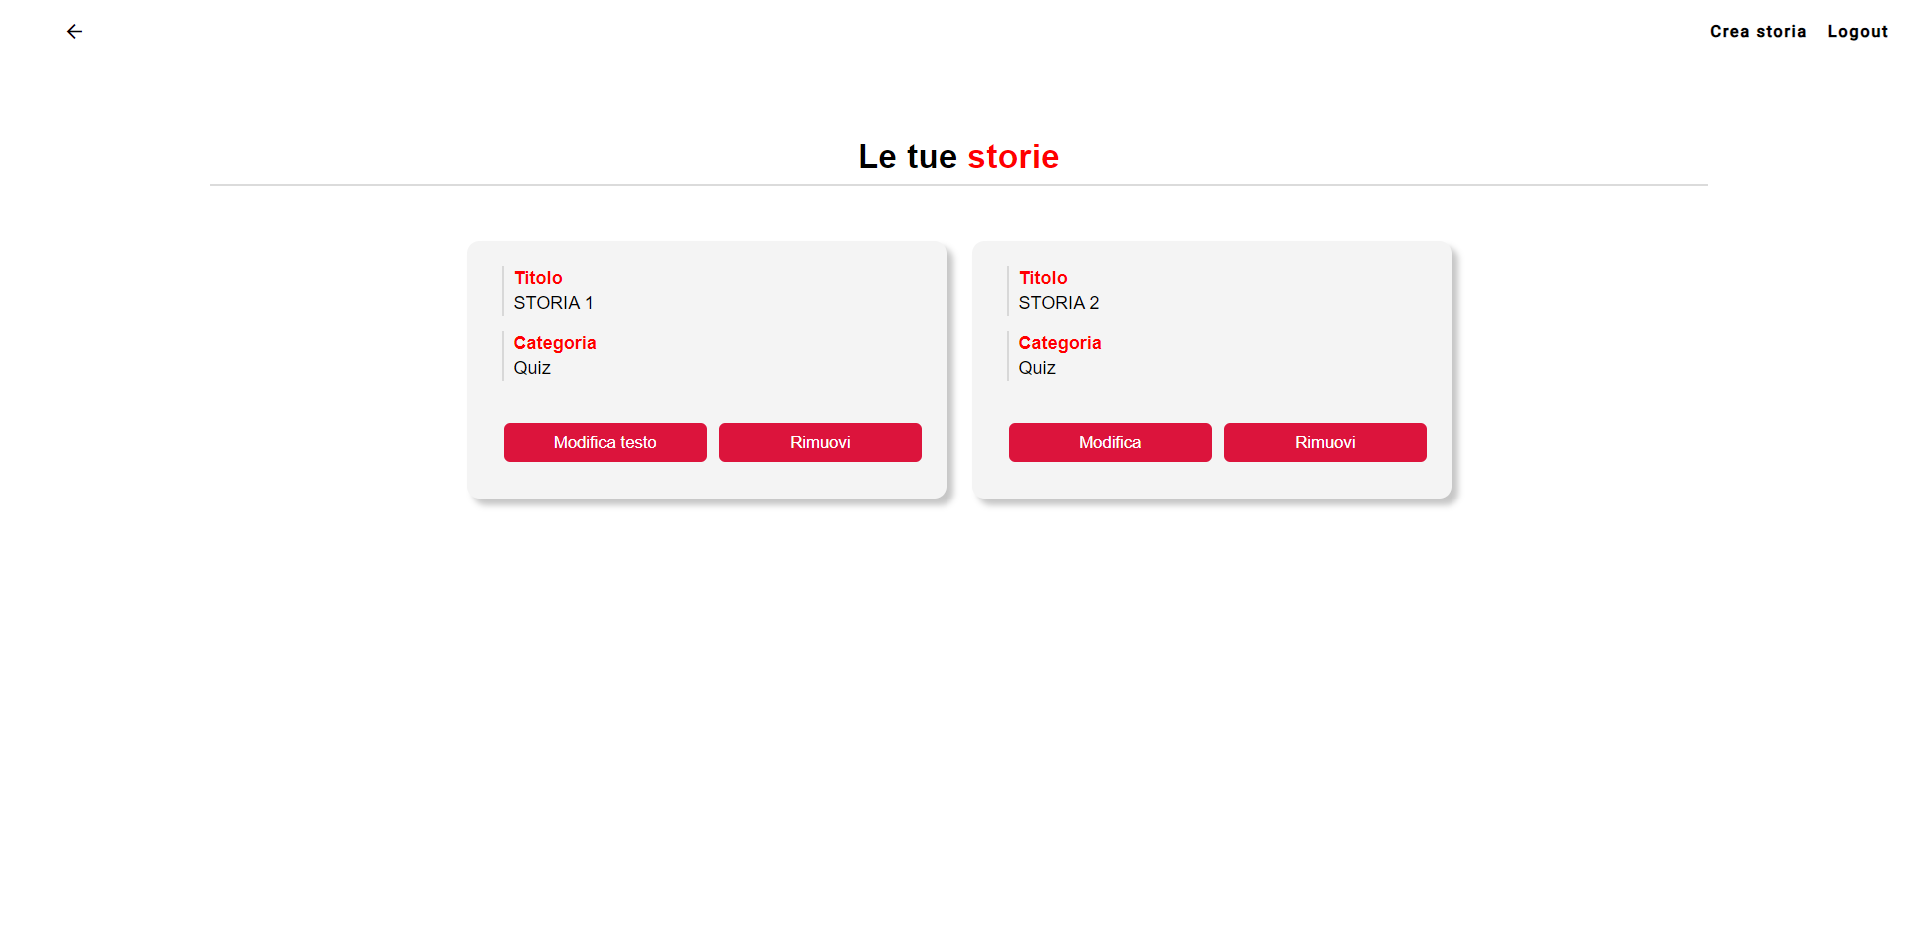
\includegraphics[width=0.8\textwidth]{foto9.png}
\end{center}

\subsection*{Form creazione storia}
Sezione che permette la \textit{creazione} di una storia. È necessario inserire il titolo e la categoria.
\begin{center}
    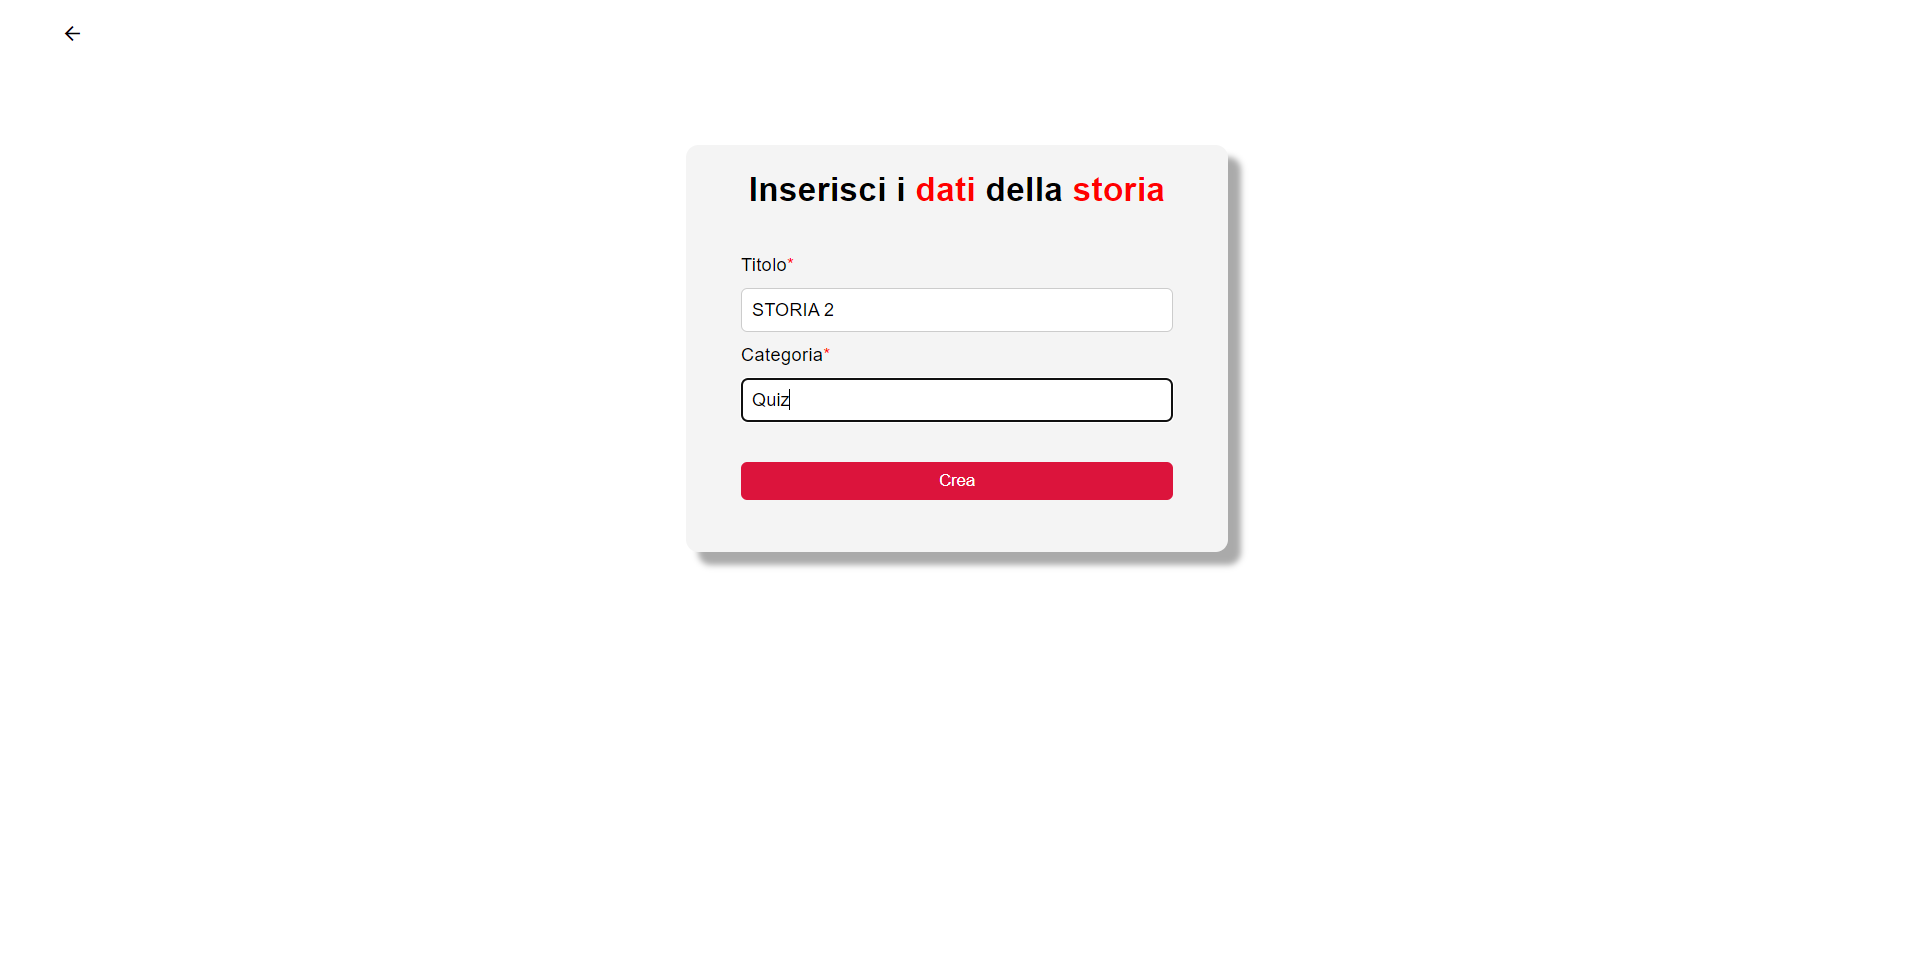
\includegraphics[width=0.8\textwidth]{foto10.png}
\end{center}

\subsection*{Scenari}
Sezione che consente la \textit{gestione} di una storia specifica. Permette di visualizzare gli scenari appartenenti alla storia. Ad ognuno di essi sono associate le relative informazioni e due bottoni, utilizzati per l'accesso alla \textit{gestione} delle scelte e per la \textit{cancellazione} dello scenario. È presente una navbar che permette di salvare la storia e accedere alle sezioni relative alla \textit{creazione} di uno scenario, e infine alla \textit{gestione} degli oggetti.
\begin{center}
    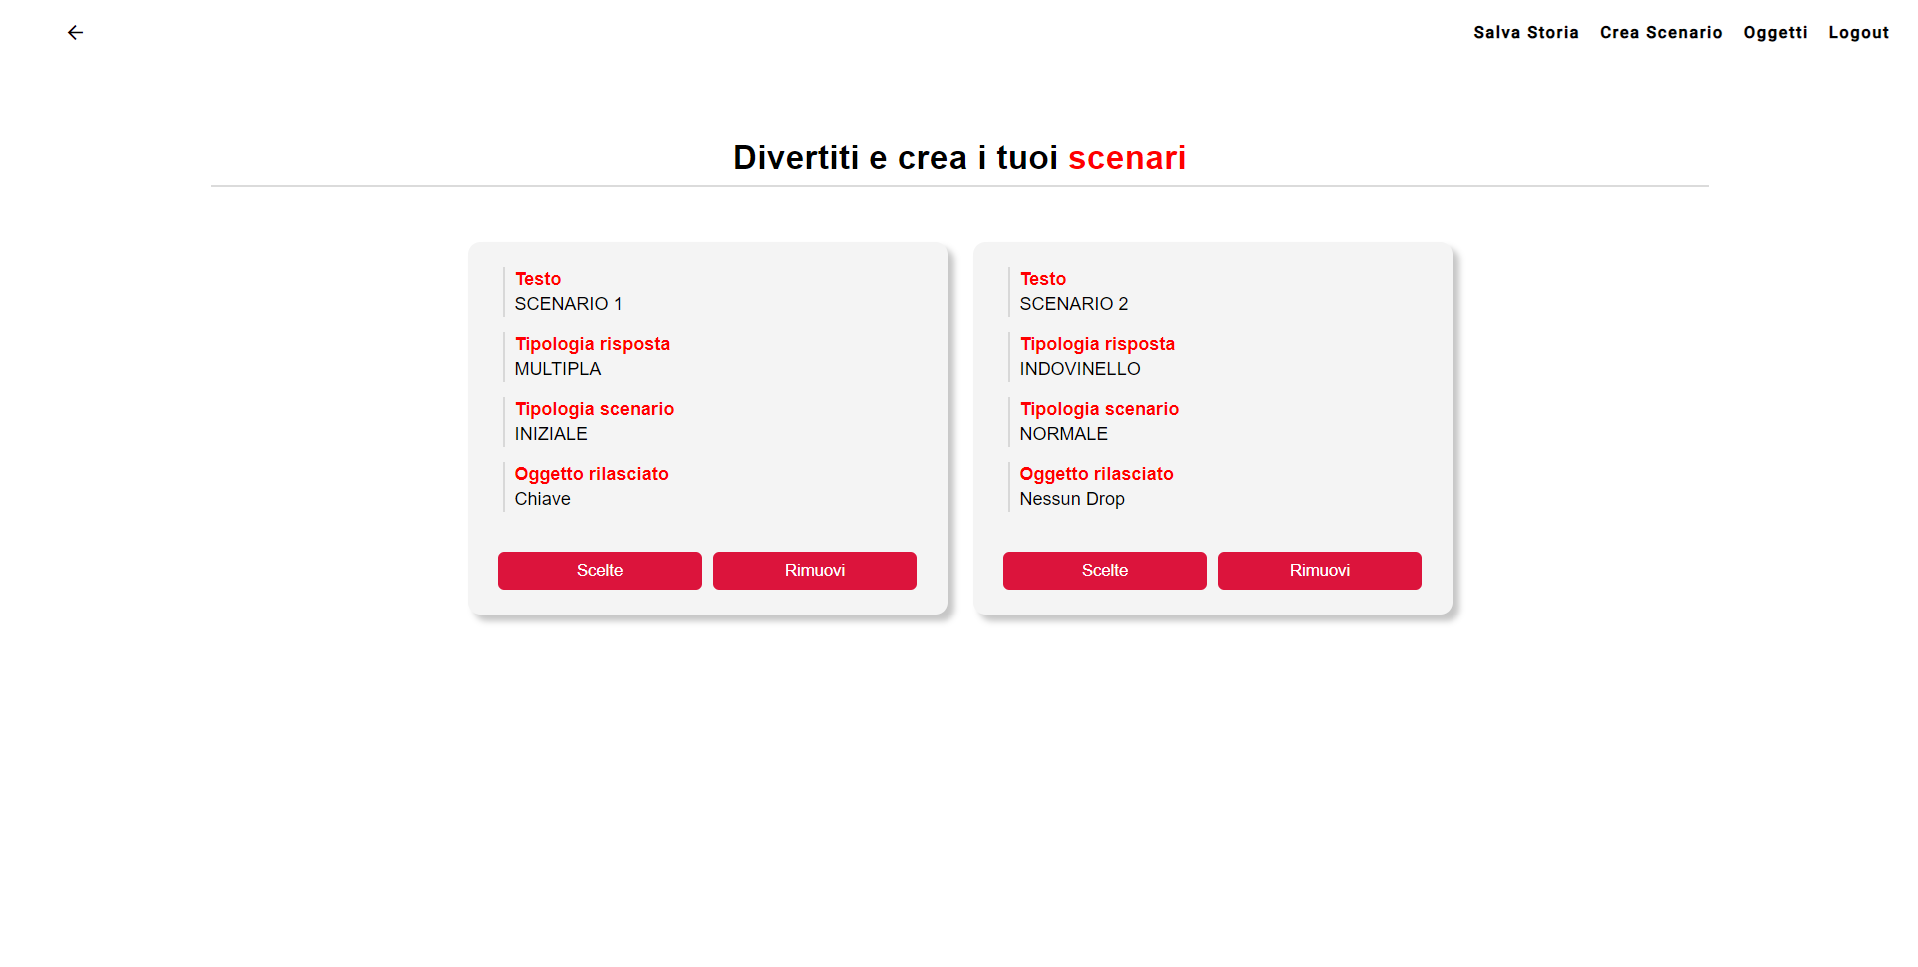
\includegraphics[width=0.8\textwidth]{foto11.png}
\end{center}
Una volta effettuato il salvataggio della storia, sarà possibile solo modificare i testi relativi ad essa.
\begin{center}
    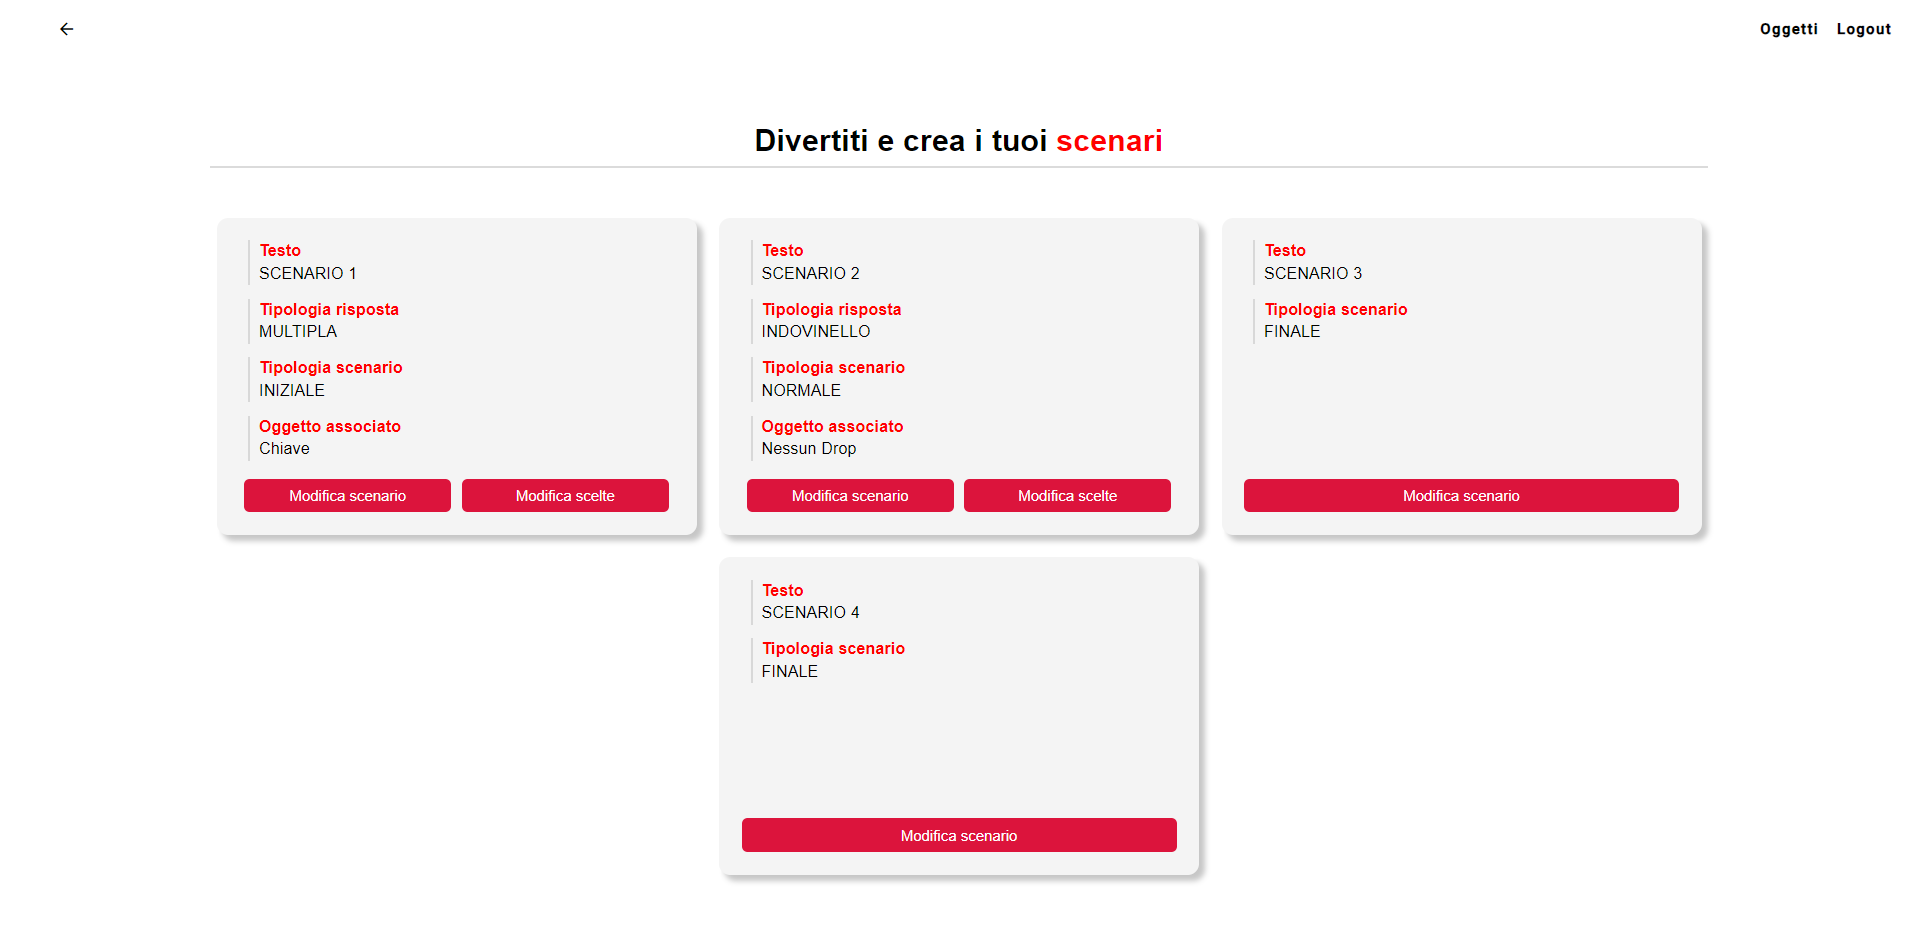
\includegraphics[width=0.8\textwidth]{foto12.png}
\end{center}

\subsection*{Form creazione scenario}
Sezione che permette la \textit{creazione} di uno scenario. È necessario inserire i dati relativi ad esso, quindi il testo, la tipologia di scenario, la tipologia di risposta ed infine indicare la presenza o meno del drop di un oggetto.\vspace*{7pt}\\
\textit{Nota bene}: è necessario aver già creato l'oggetto che si vuole far rilasciare dallo scenario.
\begin{center}
    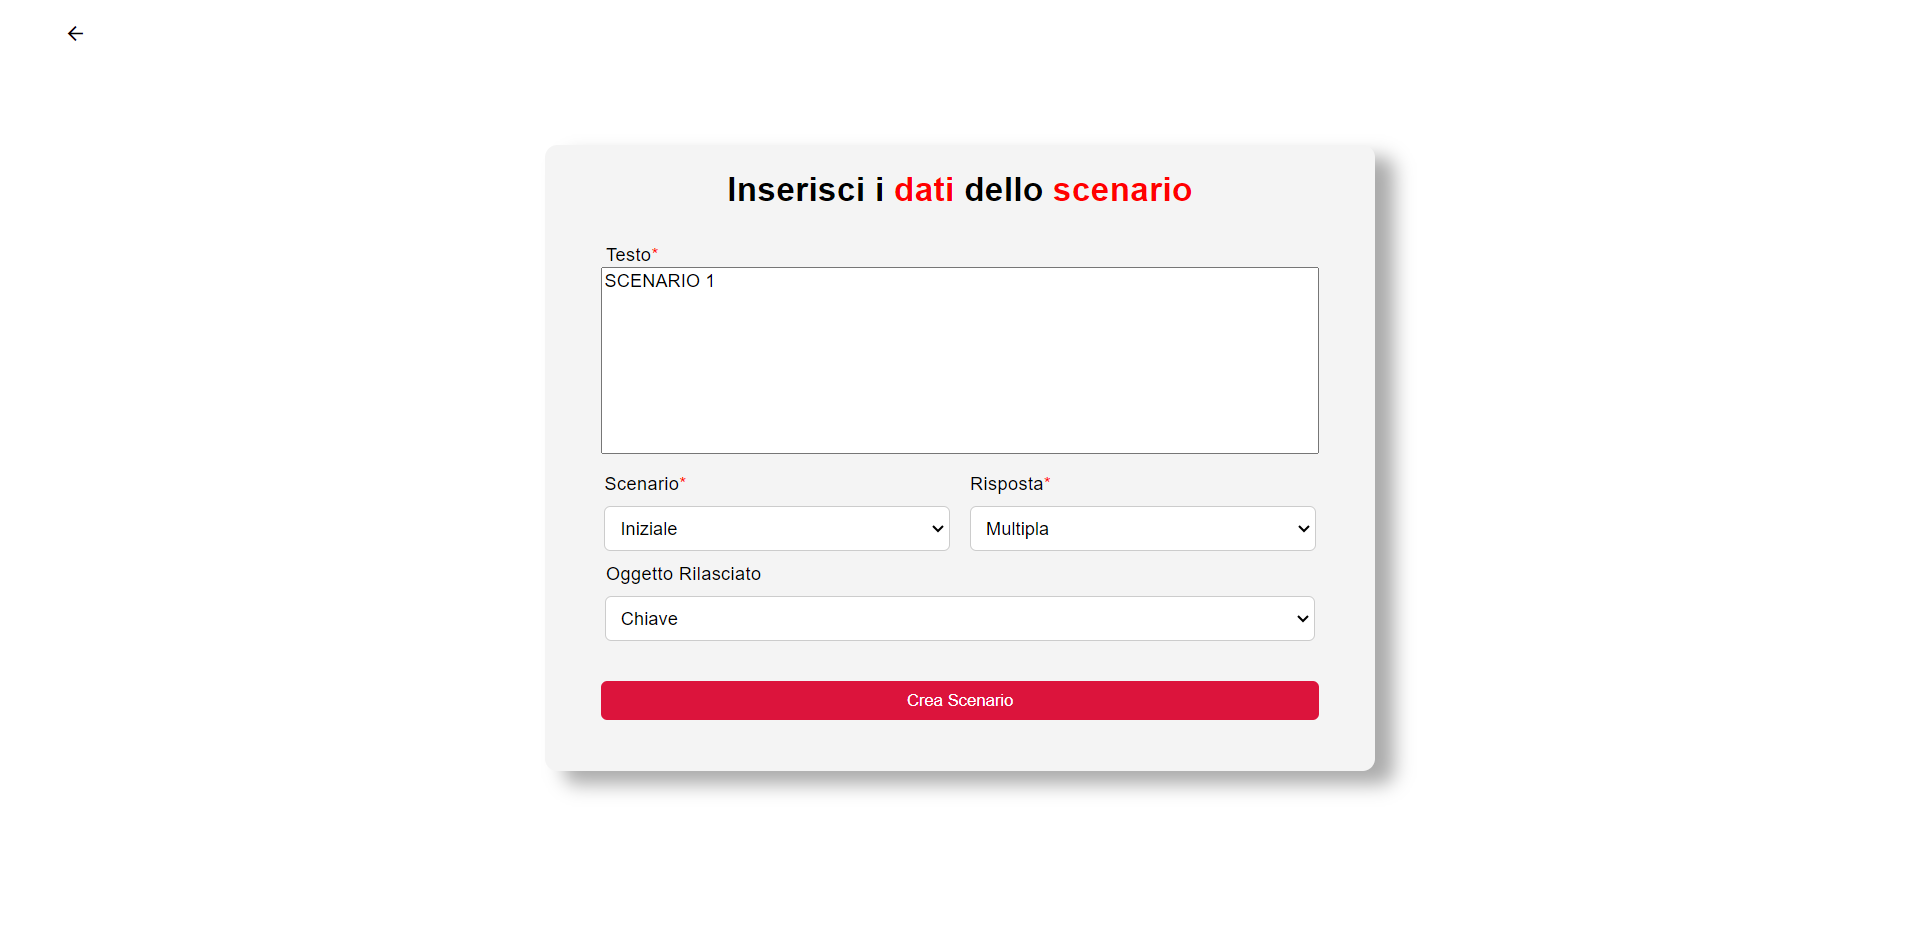
\includegraphics[width=0.8\textwidth]{foto13.png}
\end{center}

\subsection*{Indovinello}
Sezione che permette la \textit{gestione} della risposta ad un indovinello. È possibile visualizzare i dati relativi a quest'ultimo, quindi il testo, la risposta associata ed infine gli scenari destinazione in seguito alla risposta corretta piuttosto che alla risposta errata.
\begin{center}
    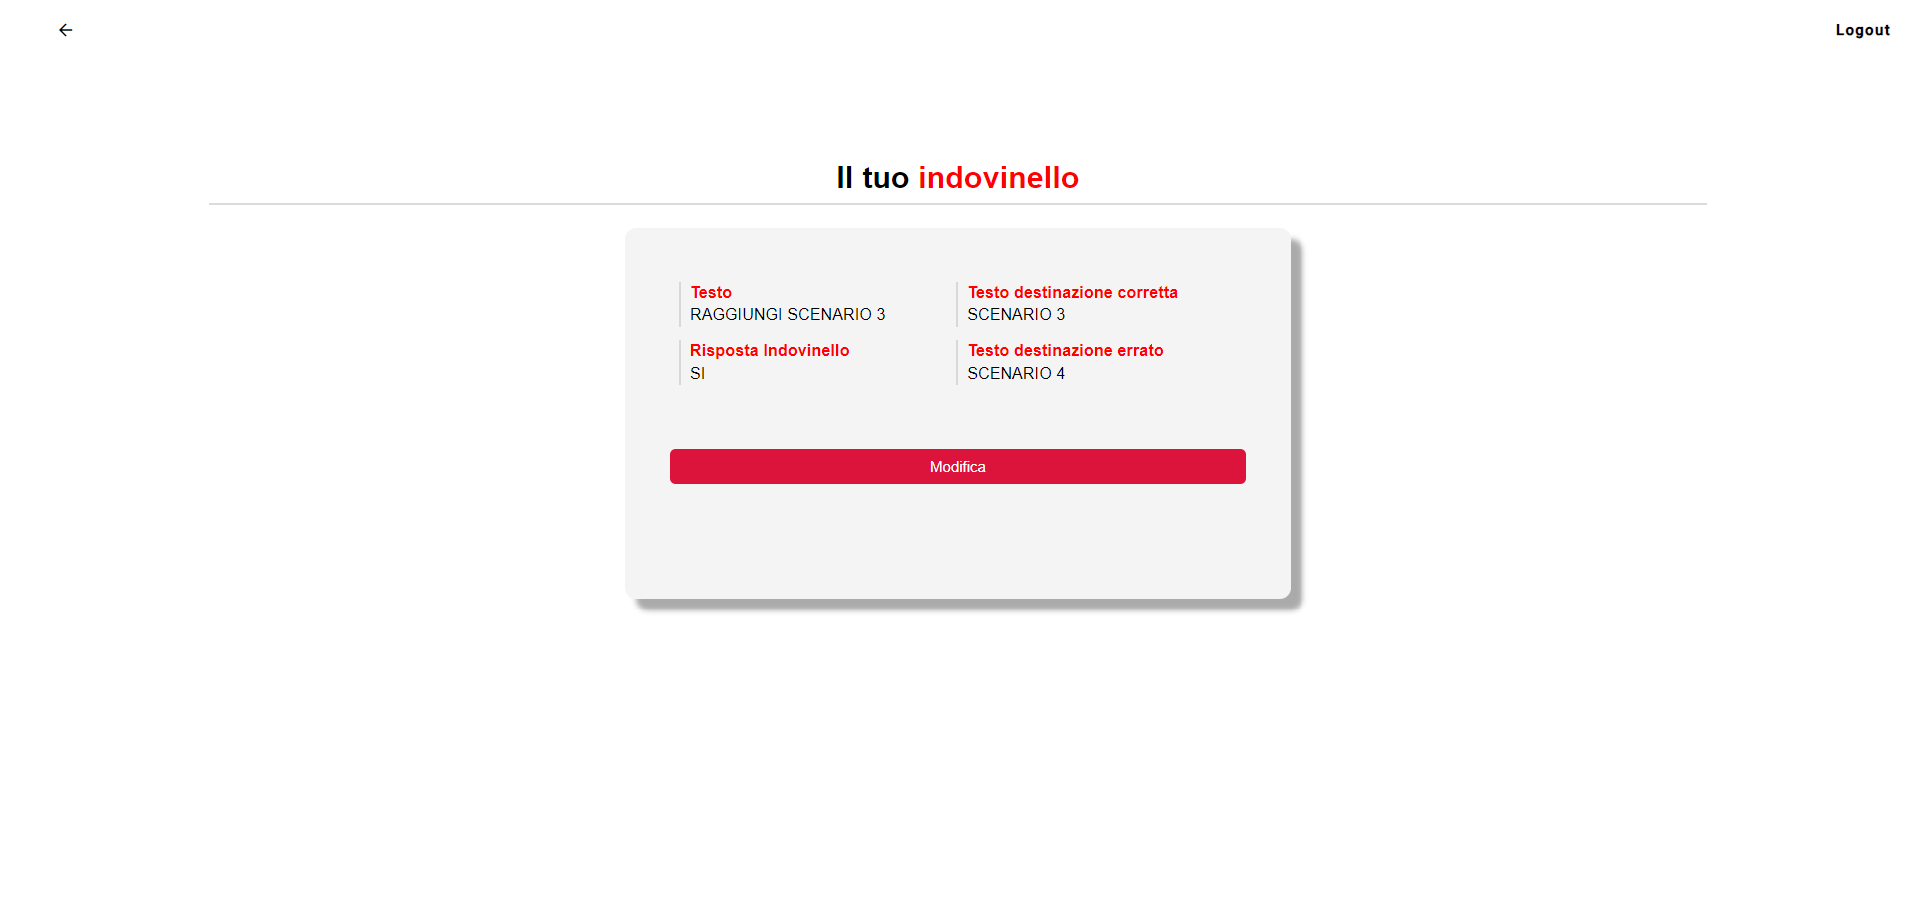
\includegraphics[width=0.8\textwidth]{foto14.png}
\end{center}
È possibile cancellare l'indovinello, se presente, e attraverso navbar ci sarà la possibilità di crearne uno nuovo.
\begin{center}
    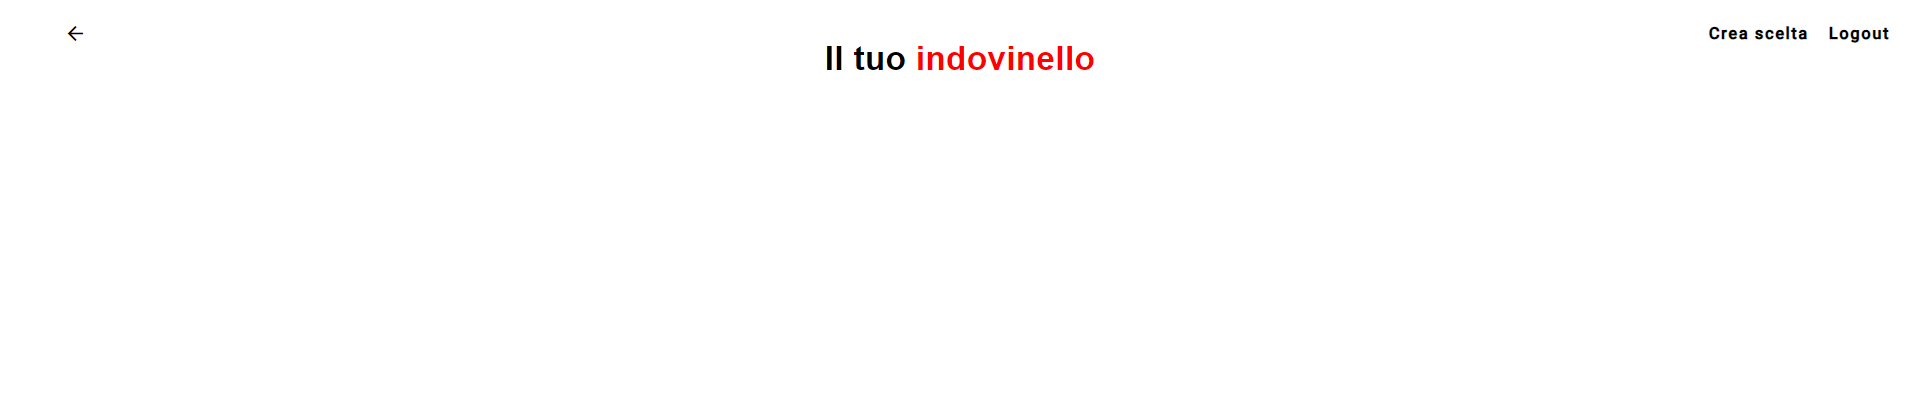
\includegraphics[width=0.8\textwidth]{foto15.png}
\end{center}

\subsection*{Form creazione indovinello}
Sezione che permette la \textit{creazione} della risposta ad un indovinello. È necessario inserire il testo del quesito, la risposta attesa ed infine gli scenari di destinazione in seguito alla risposta corretta piuttosto che alla risposta errata.
\begin{center}
    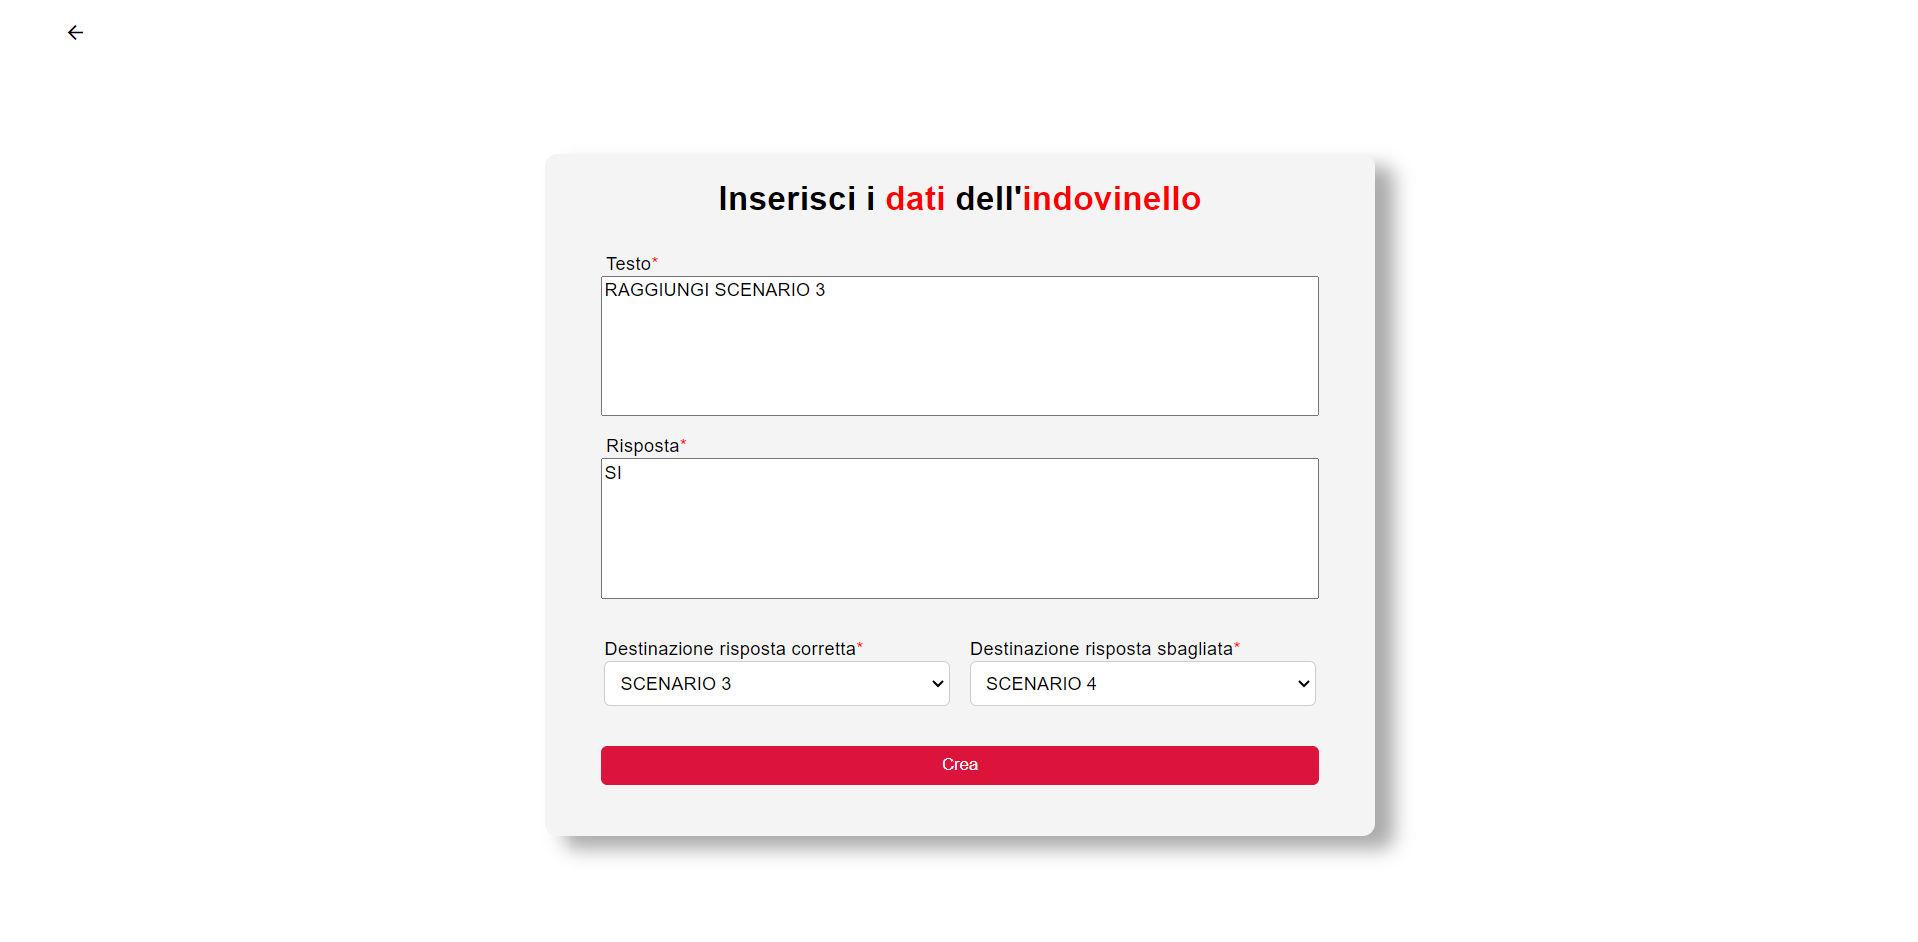
\includegraphics[width=0.8\textwidth]{foto16.png}
\end{center}

\subsection*{Scelta multipla}
Sezione che permette la \textit{gestione} delle risposte ad una domanda a scelta multipla. È possibile visualizzare i dati relativi alle opzioni già presenti, quindi il testo, lo scenario successivo alla risposta, e la presenza o meno di un oggetto richiesto.\vspace*{7pt}\\
\textit{Nota bene}: è necessario aver già creato l'oggetto richiesto.\vspace*{7pt}\\
È possibile inoltre cancellare le opzioni, se presenti, e attraverso navbar ci sarà la possibilità di crearne nuove.
\begin{center}
    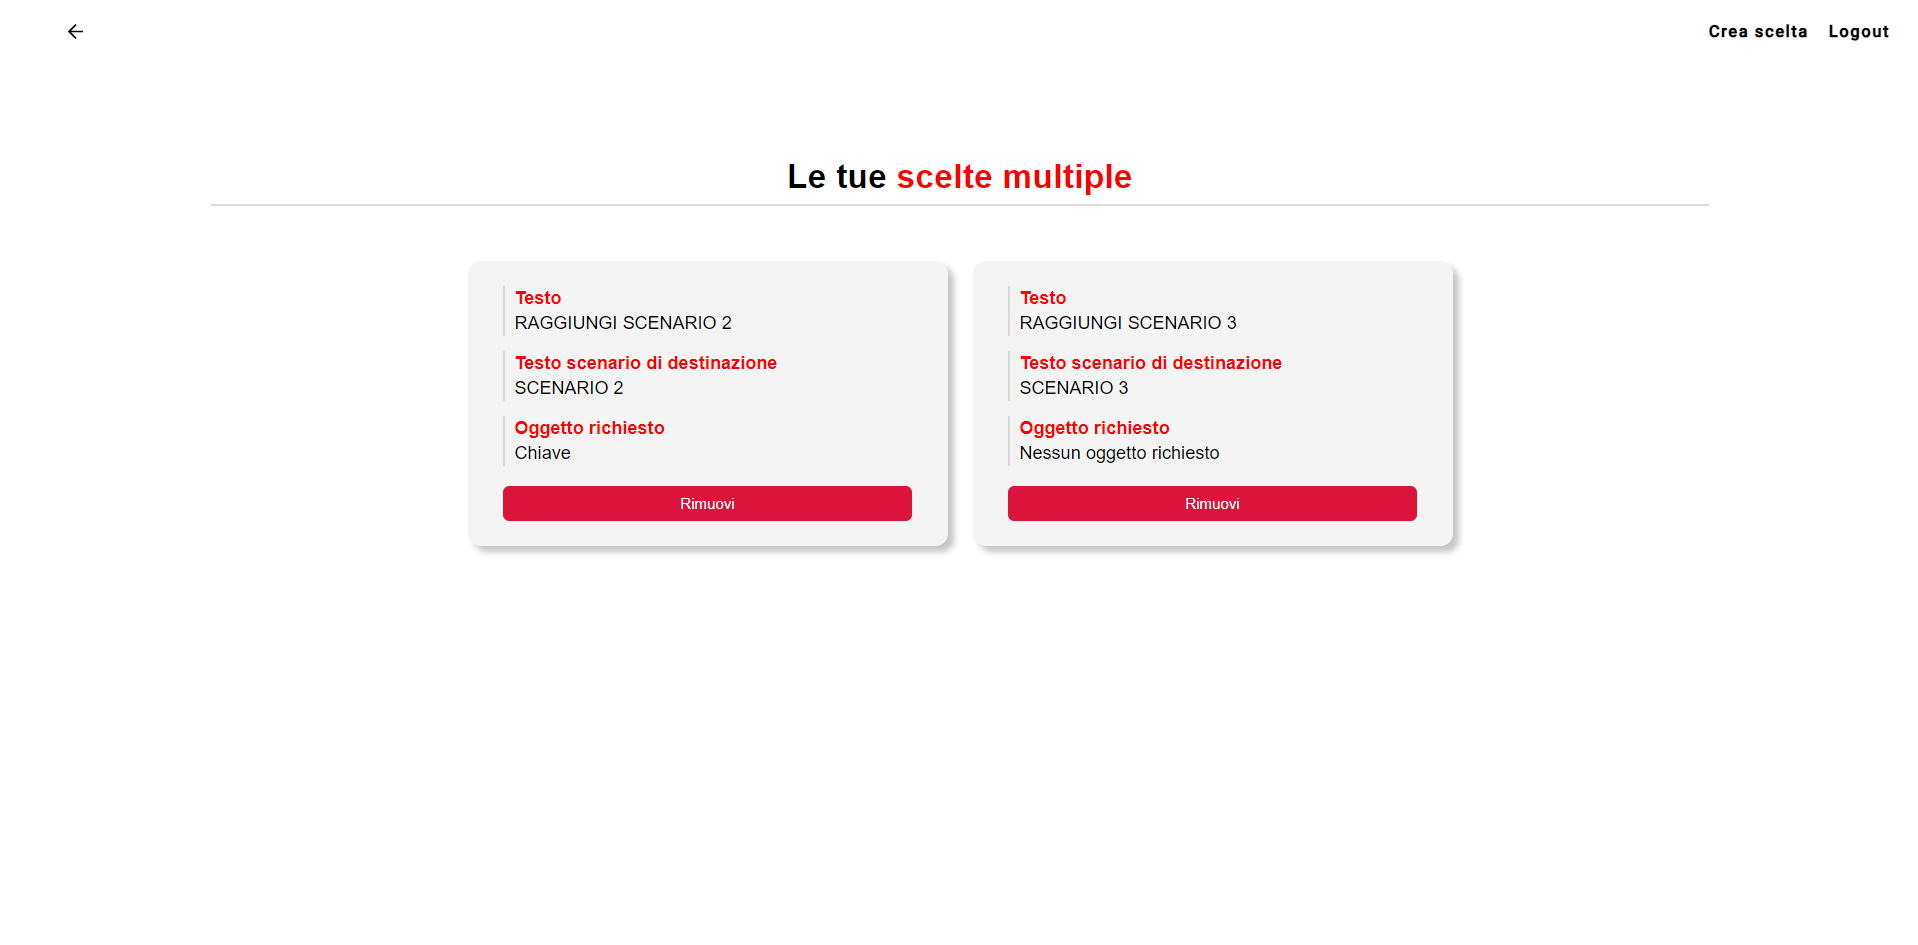
\includegraphics[width=0.8\textwidth]{foto17.png}
\end{center}

\subsection*{Form creazione multipla}
Sezione che permette la \textit{creazione} della risposta ad una domanda a scelta multipla. È necessario inserire il testo del quesito, lo scenario successivo alla risposta, e la presenza o meno di un oggetto richiesto.
\begin{center}
    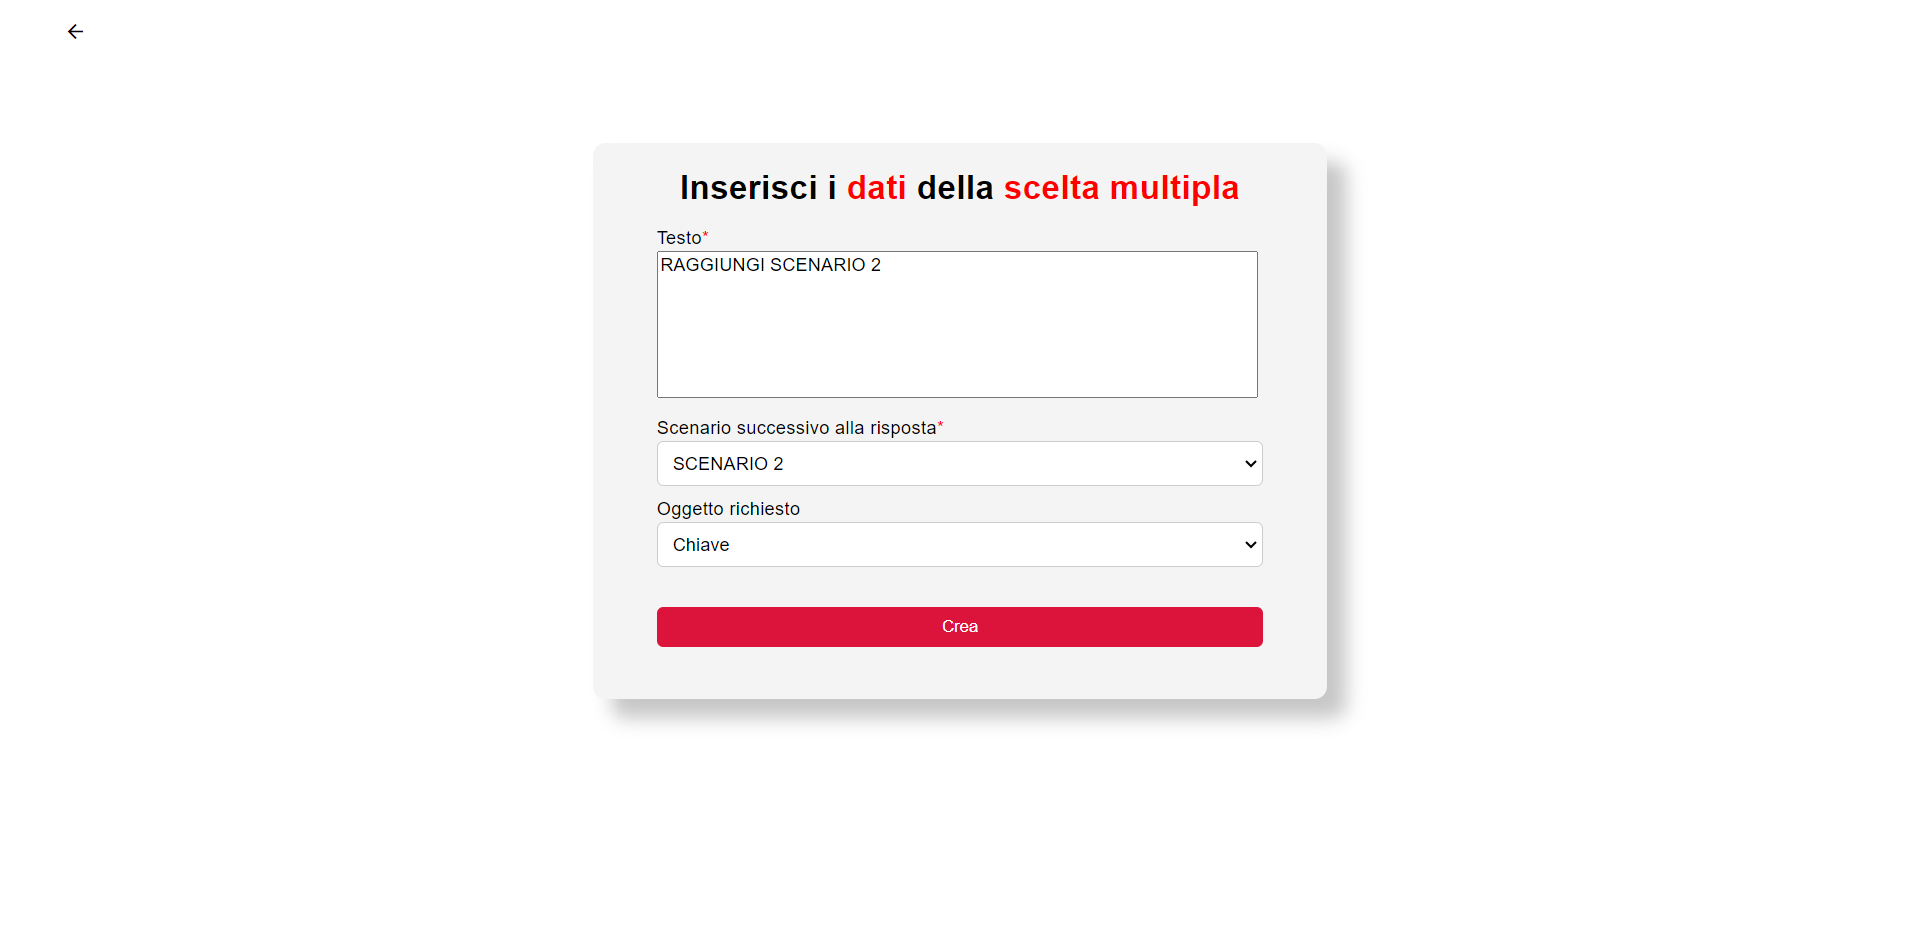
\includegraphics[width=0.8\textwidth]{foto18.png}
\end{center}

\subsection*{Oggetti}
Sezione che permette la \textit{gestione} degli oggetti di una storia. È possibile visualizzare i dati relativi ad ognuno, quindi il titolo e la descrizione, ed un bottone che permette la cancellazione. Attraverso navbar ci sarà la possibilità di creare nuovi oggetti.
\begin{center}
    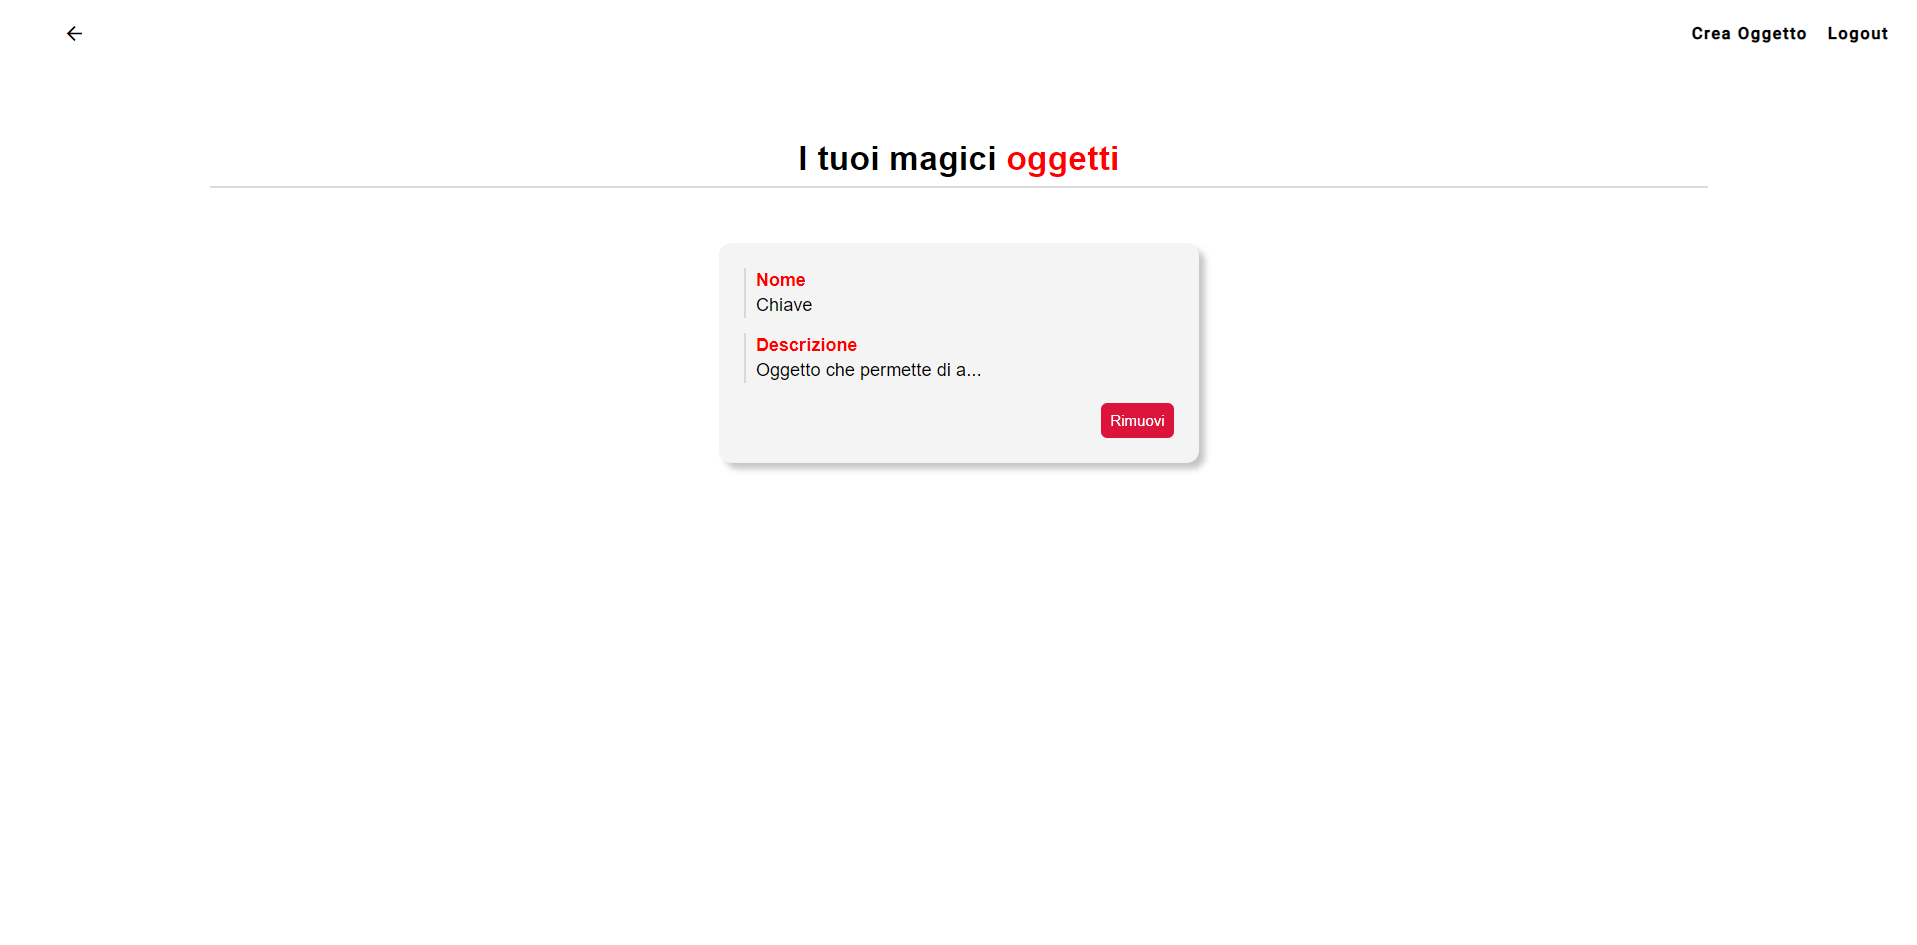
\includegraphics[width=0.8\textwidth]{foto19.png}
\end{center}

\subsection*{Form creazione oggetti}
Sezione che permette la \textit{creazione} di un oggetto. È necessario inserire i dati relativi ad esso, quindi il titolo e la descrizione.
\begin{center}
    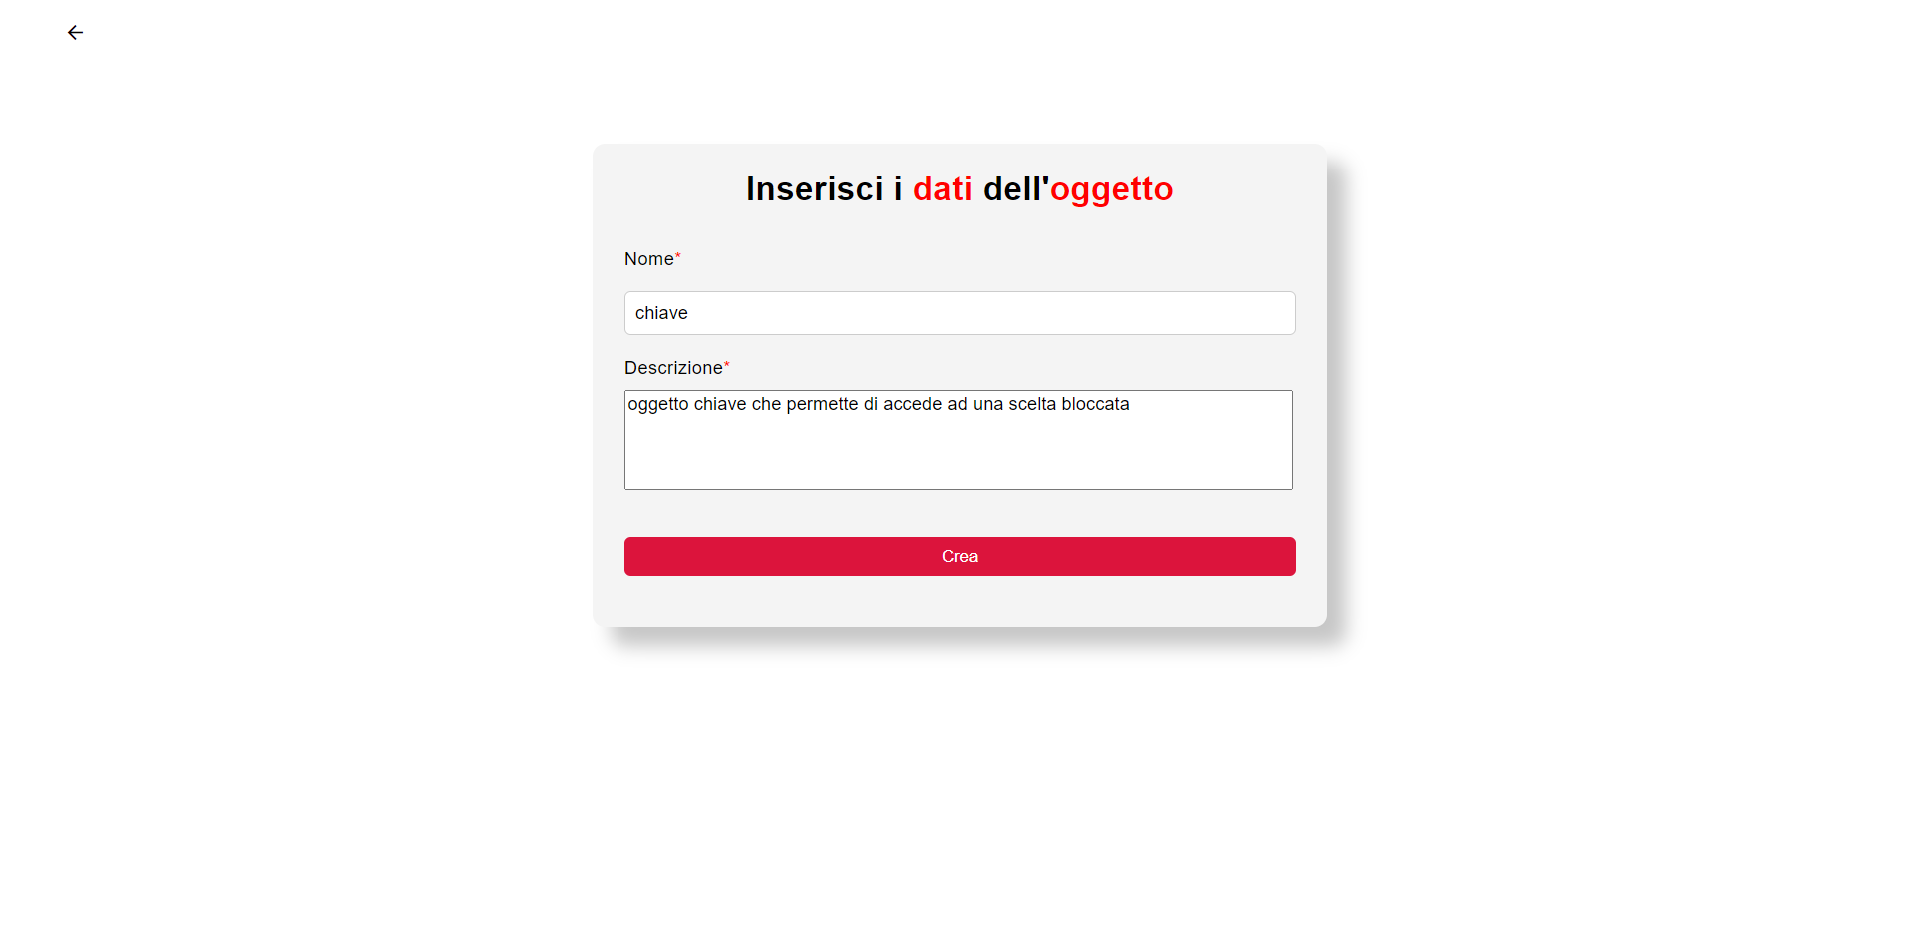
\includegraphics[width=0.8\textwidth]{foto20.png}
\end{center}

\subsection*{Storie giocabili}
Sezione che permette la \textit{selezione} della storia da giocare. È possibile visualizzare tutte le storie giocabili con le varie informazioni, permettendo la ricerca attraverso dei filtri.
\begin{center}
    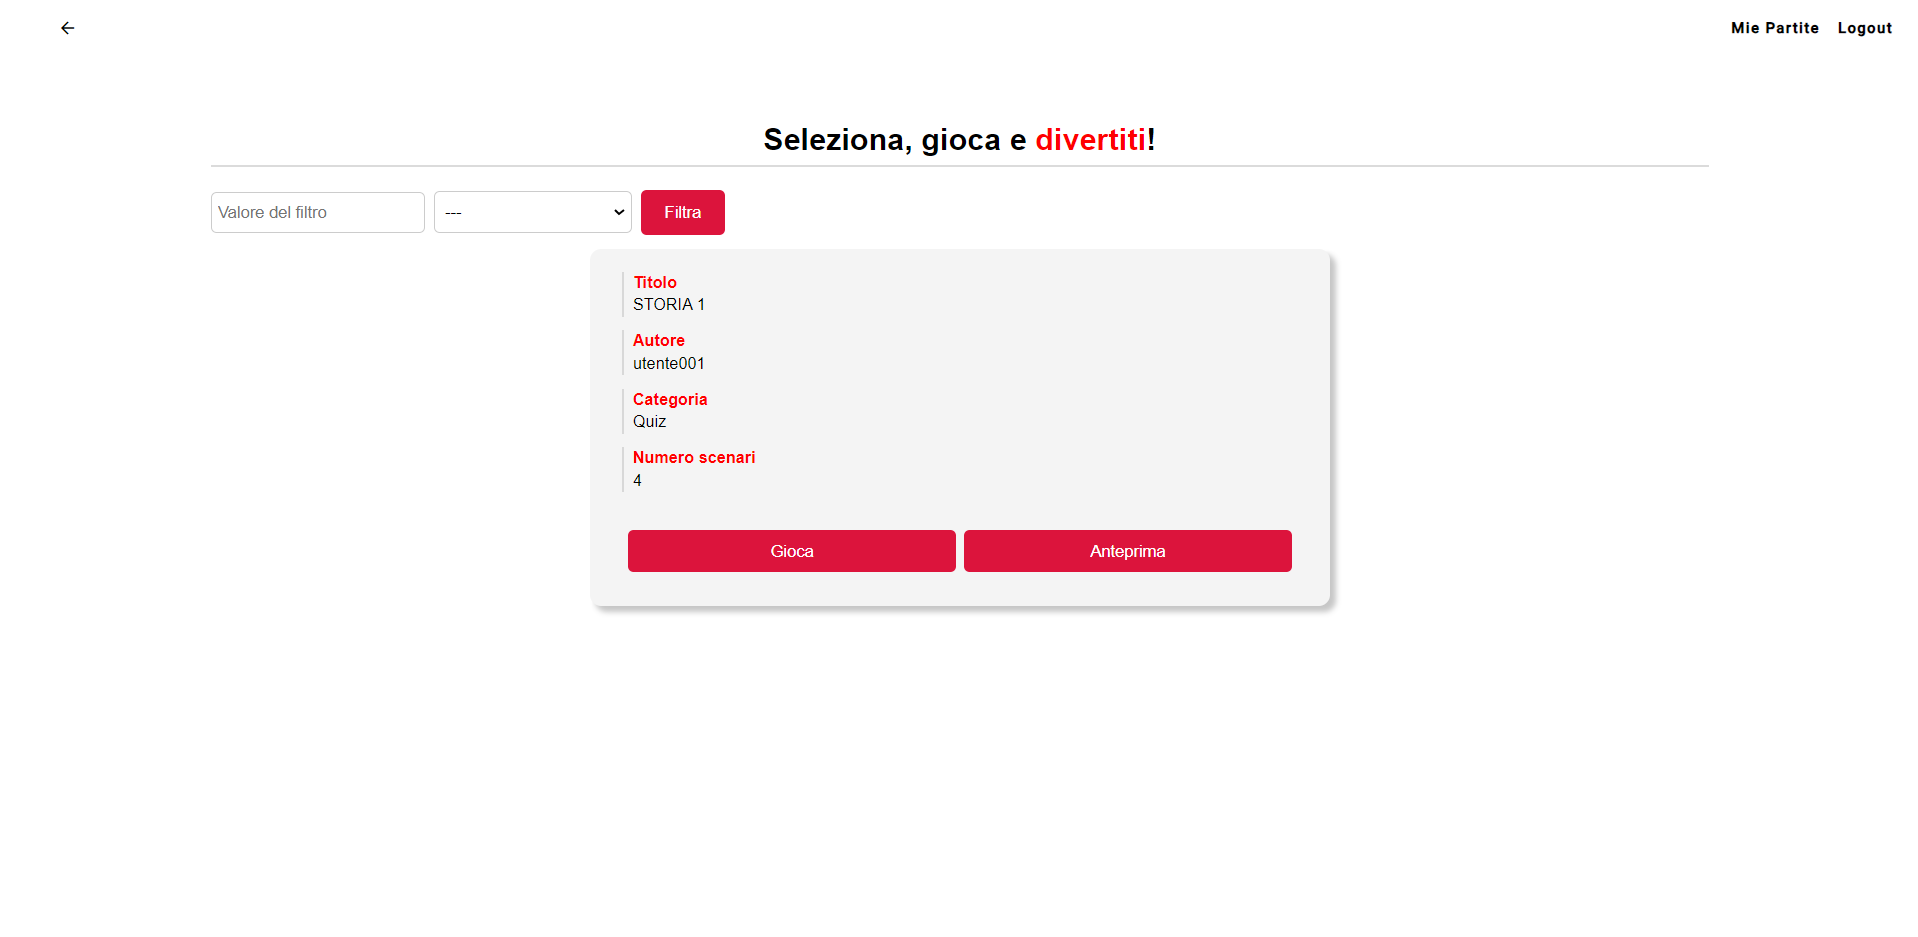
\includegraphics[width=0.8\textwidth]{foto21.png}
\end{center}
Per ogni storia presente ci sarà la possibilità di \textit{avviare} la partita, o in alternativa di \textit{visualizzare} l'\textit{anteprima} di essa.
\begin{center}
    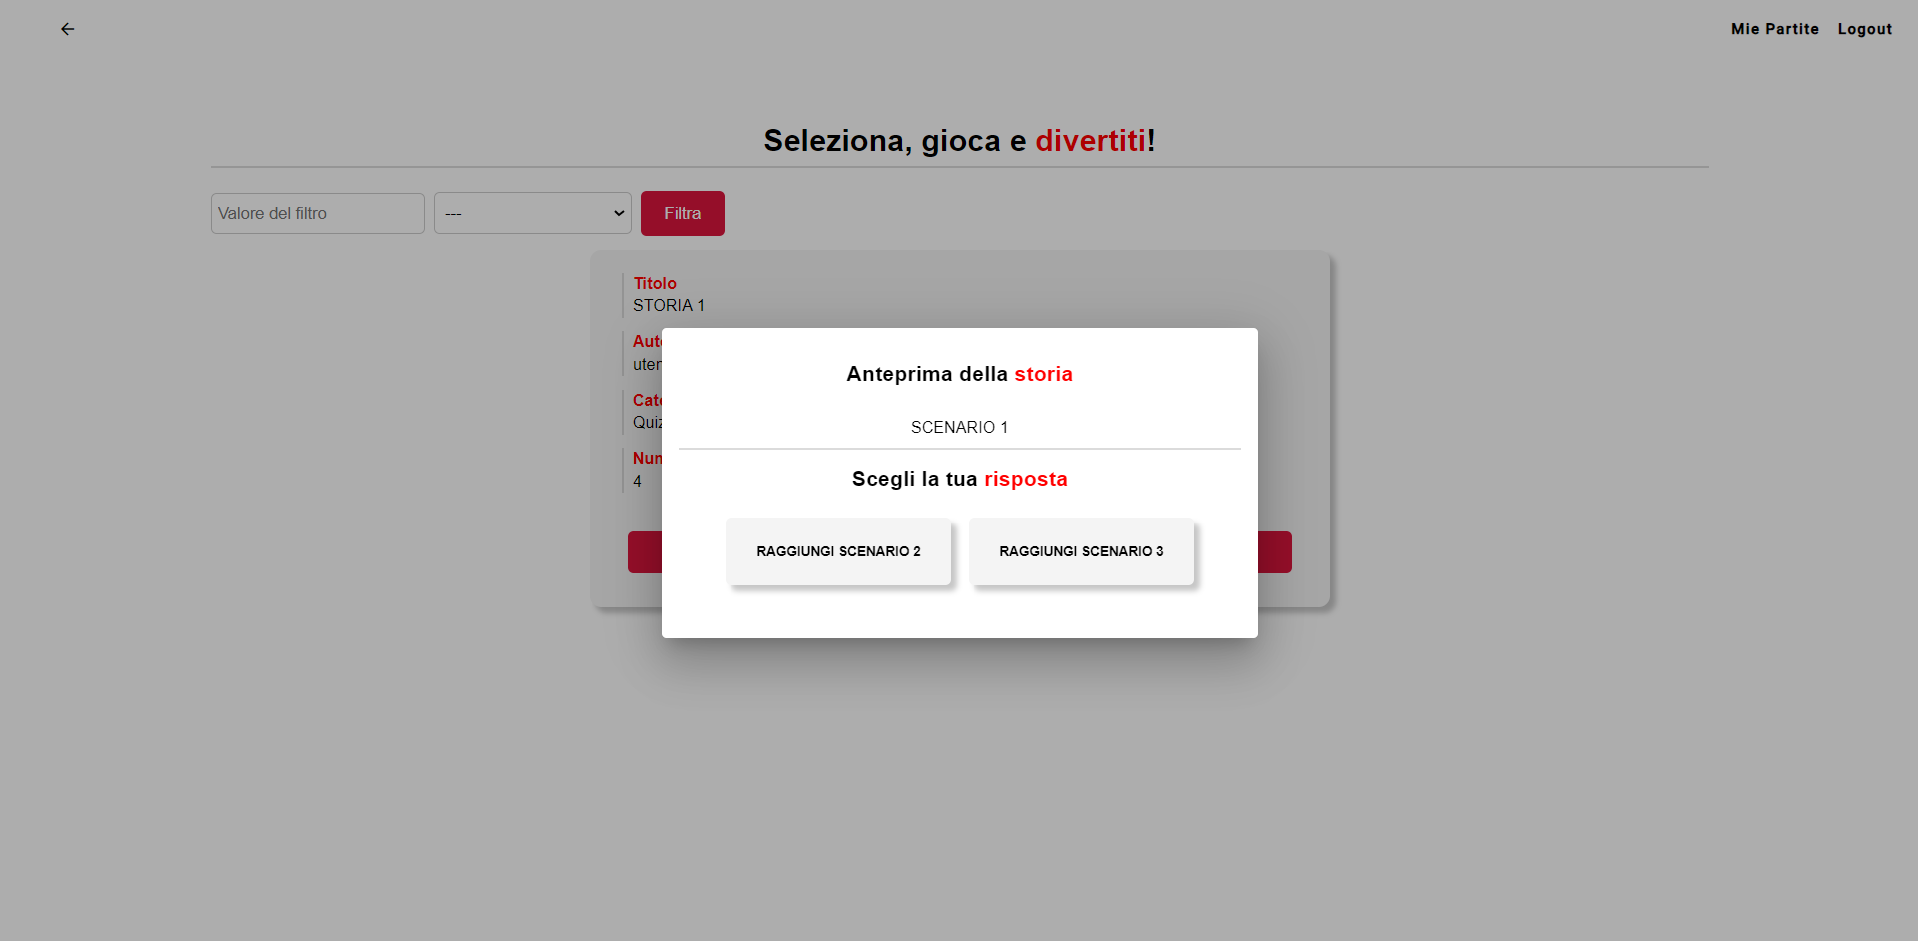
\includegraphics[width=0.8\textwidth]{foto22.png}
\end{center}

\subsection*{Gioca}
Sezione in cui avviene lo \textit{svolgimento} della partita. All'interno della schermata sarà presente il testo dello scenario ed in base alla tipologia della domanda verranno visualizzati i bottoni contenenti le opzioni di risposta piuttosto che l'area testuale per inserire la risposta all'indovinello.
\begin{center}
    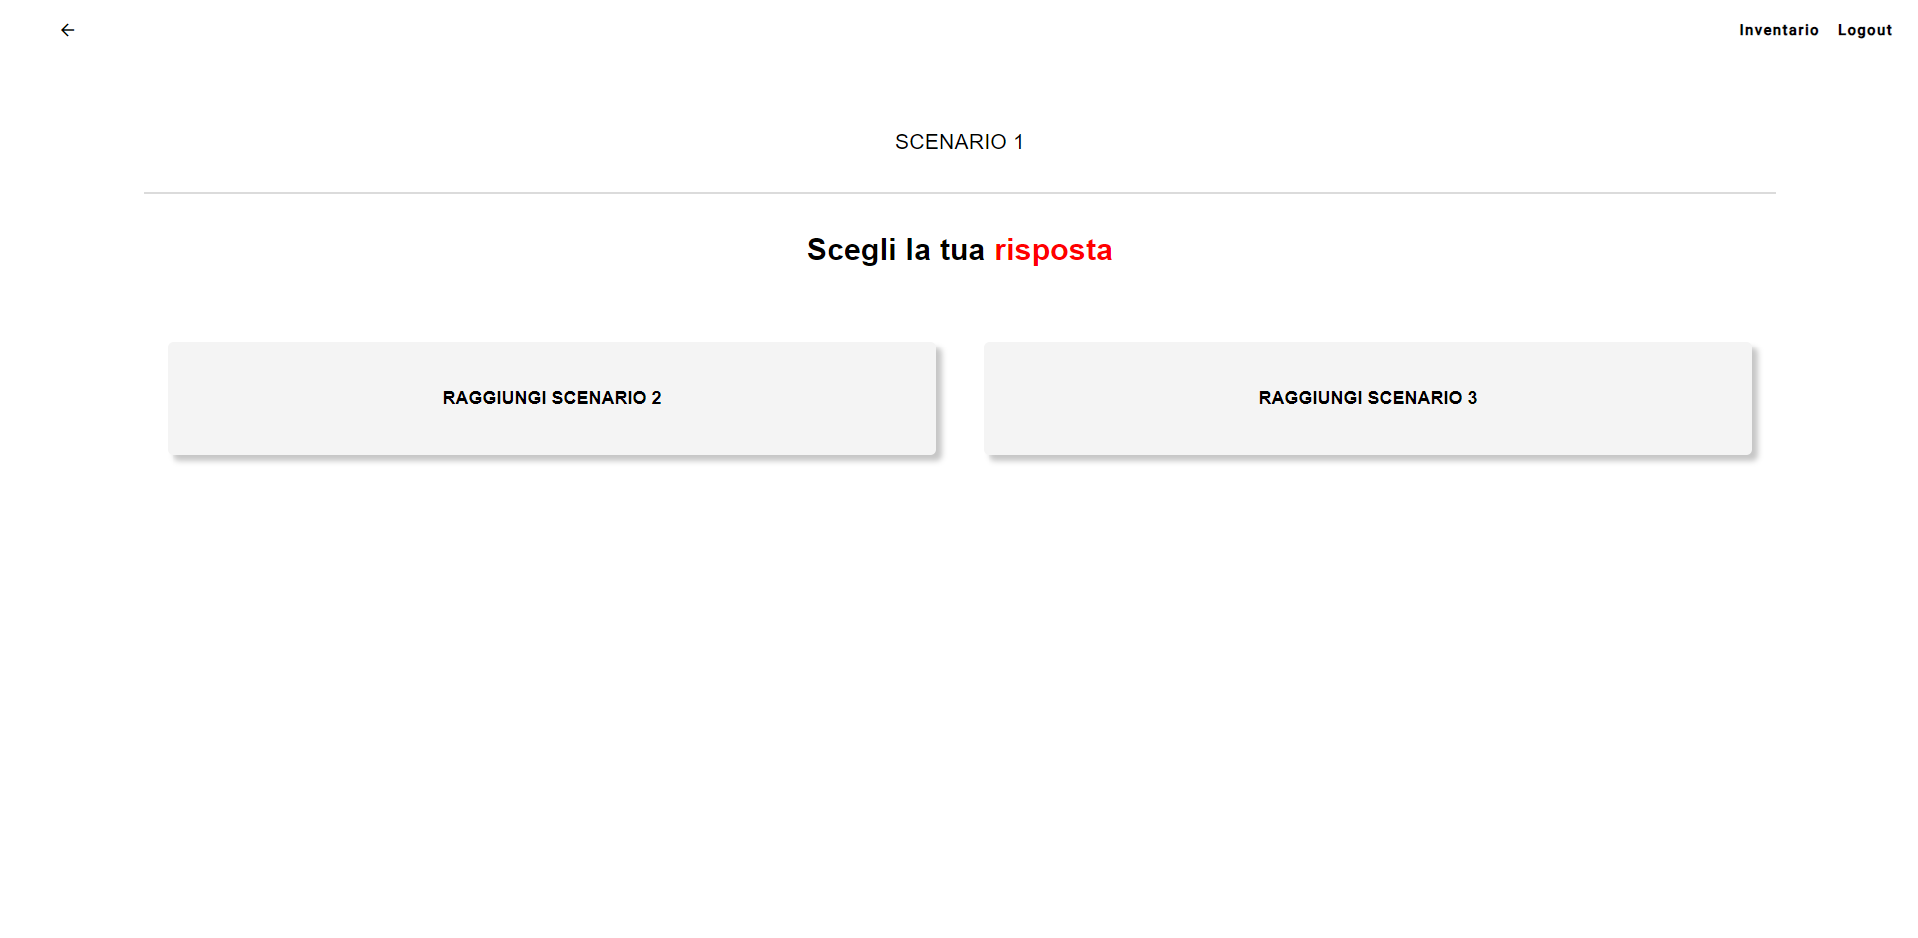
\includegraphics[width=0.8\textwidth]{foto23.png}
\end{center}
\begin{center}
    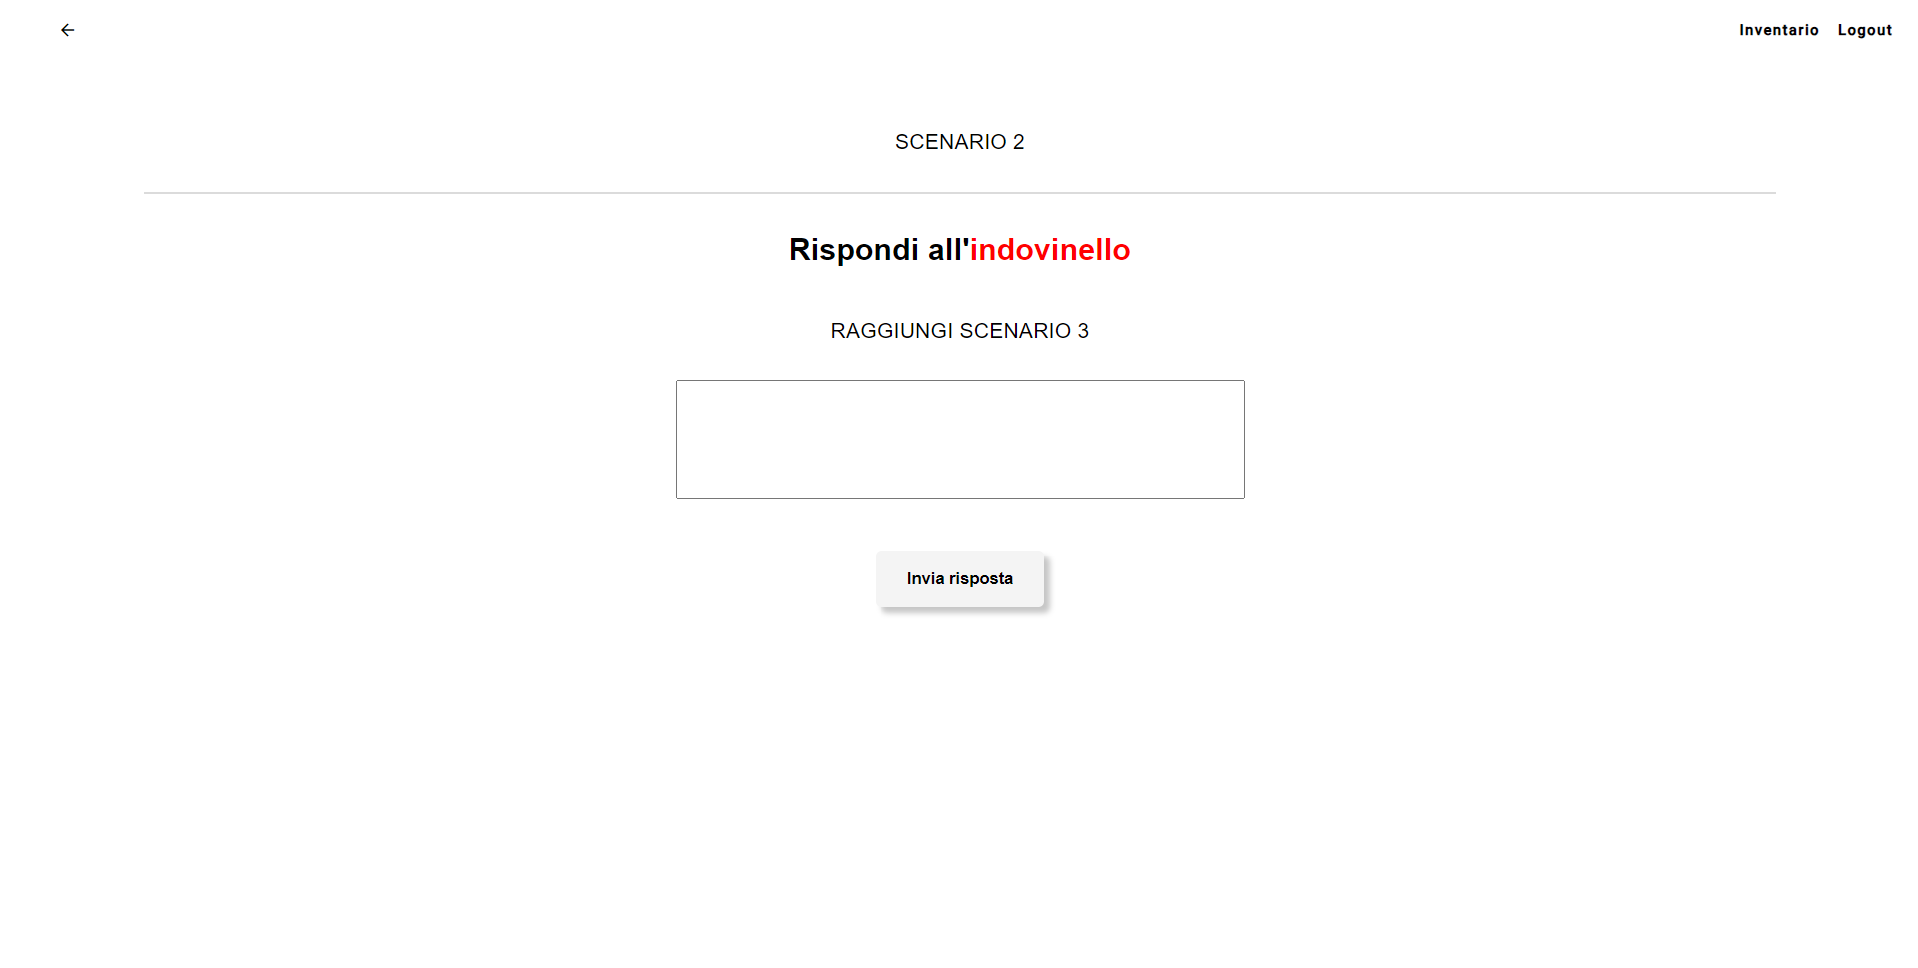
\includegraphics[width=0.8\textwidth]{foto24.png}
\end{center}
Attraverso la barra di navigazione sarà sempre possibile consultare l'\textit{inventario} della partita.
\begin{center}
    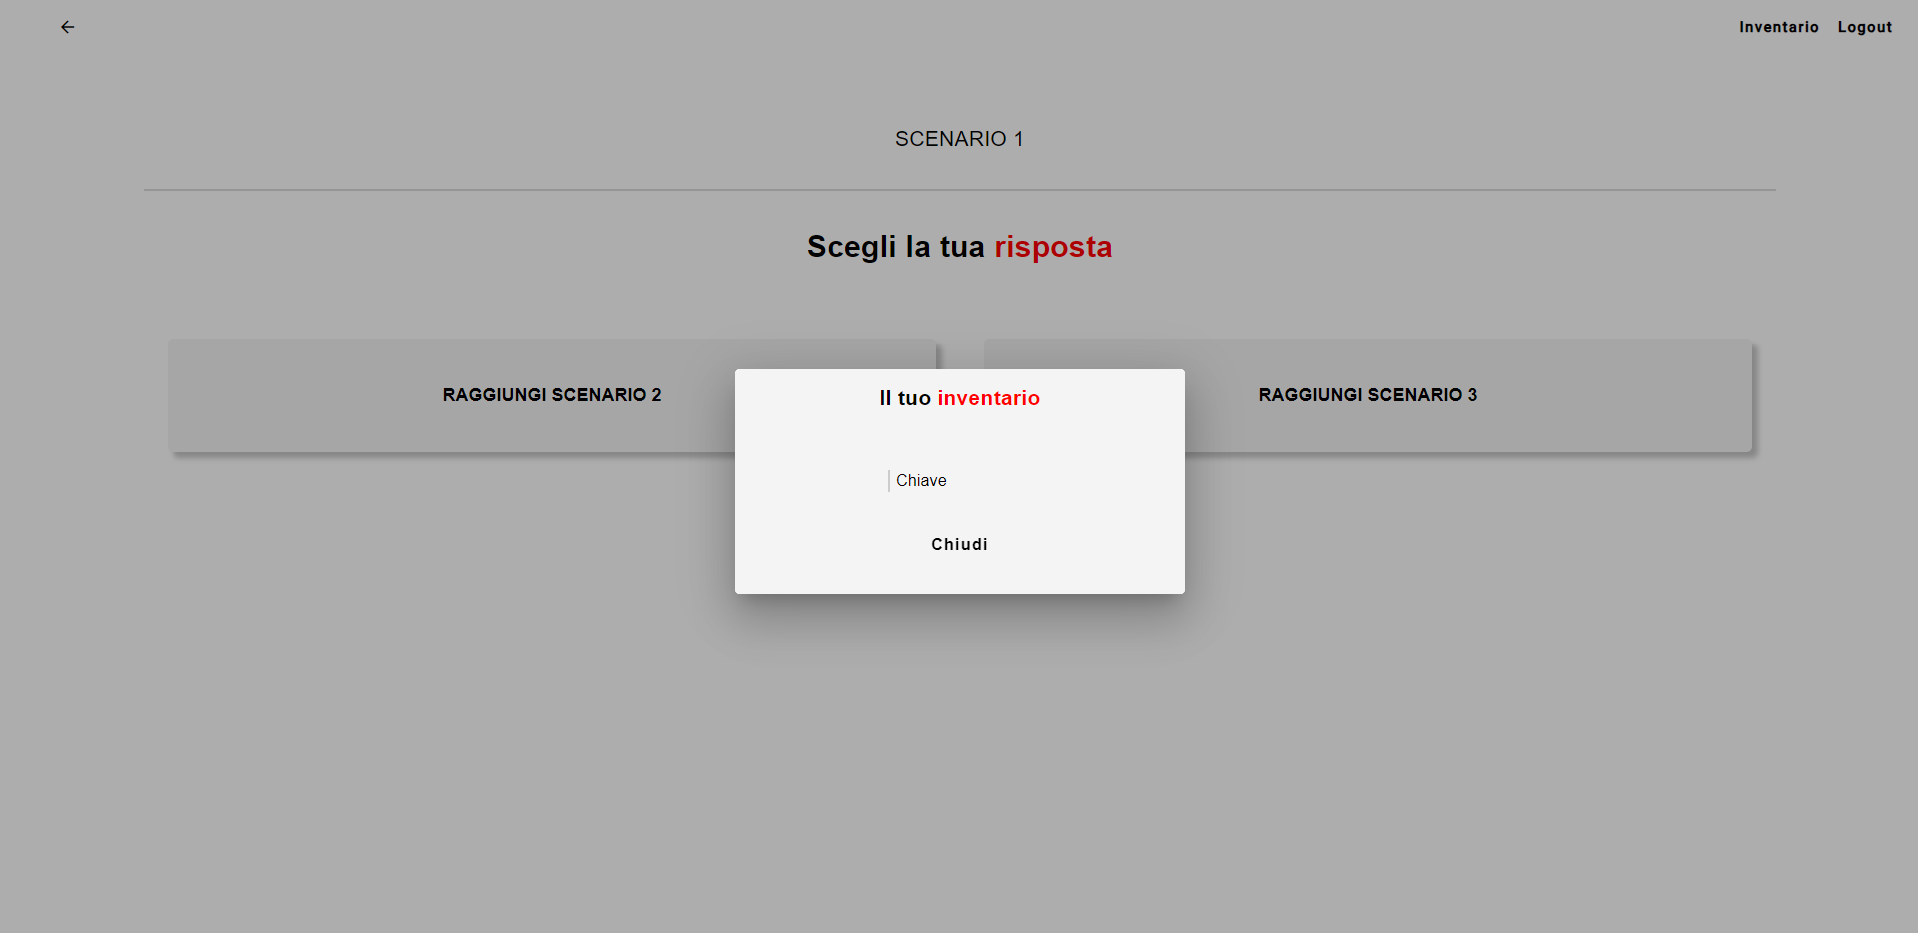
\includegraphics[width=0.8\textwidth]{foto25.png}
\end{center}

\subsection*{Partite giocate}
Sezione in cui sono presenti le partite avviate dall'utente. Per ogni partita sarà possibile riprendere la storia dallo scenario in cui era stata interrotta oppure rimuovere i dati di gioco relativi ad essa.
\begin{center}
    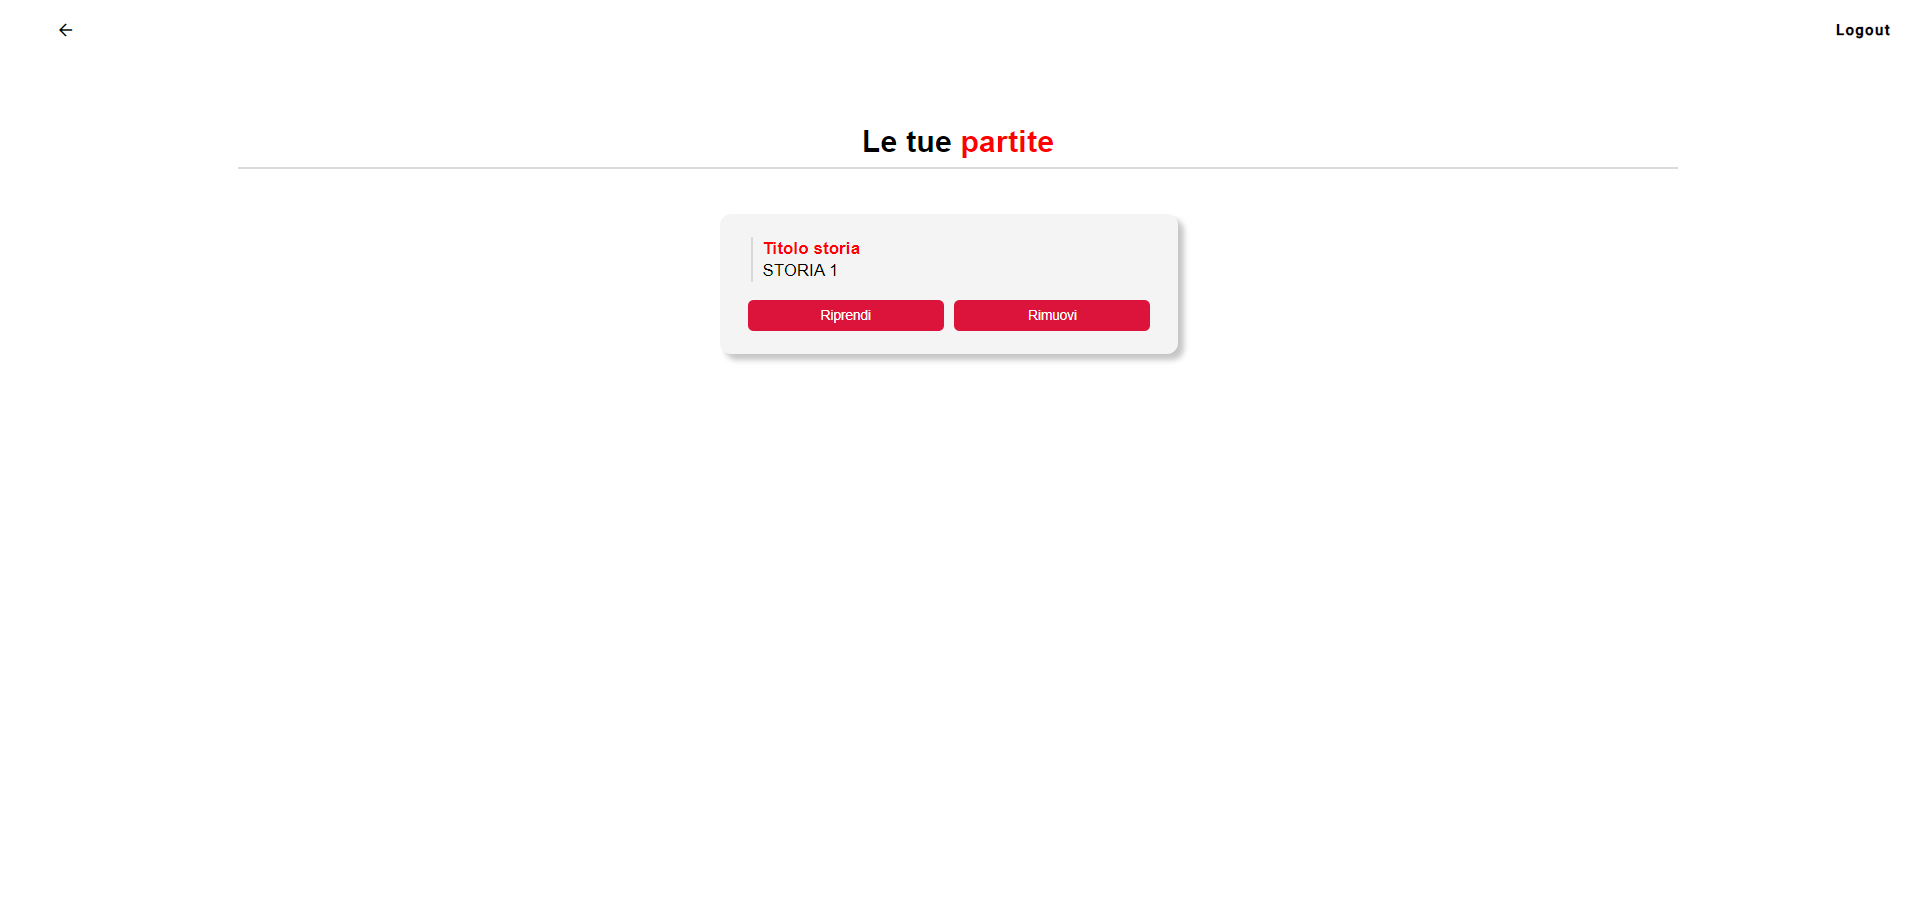
\includegraphics[width=0.8\textwidth]{foto26.png}
\end{center}

\clearpage
\section*{Manuale dello sviluppatore}

\subsection{Setup e deploy}
Unico requisito per il deploy dell'applicativo è \textbf{Docker}. Una volta scaricata la \textit{repository} da \textit{GitHub}, sarà sufficiente eseguire all'interno della cartella il comando \textbf{docker-compose up --build}; quest ultimo permetterà a \textit{Docker} di eseguire la fase di \textit{build} e successivamente di \textit{avviare} i \textit{container} relativi ai diversi servizi che compongono l'applicativo.\vspace*{7pt}\\
Per terminare l'esecuzione, eseguire all'interno della cartella precedente il comando \textbf{docker-compose down}, il quale terminerà ed eliminerà i \textit{container} dell'applicazione.\vspace*{7pt}\\
È stato scelto di utilizzare \textit{Docker} e \textit{Docker-Compose} per il deploy dell'applicativo per avere una maggiore facilità di \textit{deploy} e per permettere l'utilizzo del servizio senza dover installare in locale alcuna dipendenza software, come \textit{Maven}, \textit{NodeJS} o \textit{PostgreSQL}.\vspace*{7pt}\\
È possibile osservare all'interno della repository i \textit{Dockerfile} inerenti ai vari servizi, i quali permettono a \textit{Docker} di avviare i \textit{container}. Per ottenere un avvio simultaneo di tutti i servizi viene utilizzato un file \textit{docker-compose.yml}, il quale permette l'avvio dell'applicativo con un singolo comando.\vspace*{7pt}\\
Un esempio di \textit{Dockerfile} appartiene allo \textit{Spring Boot} del backend, il quale si suddivide in due fasi:
\vspace*{7pt}
\begin{lstlisting}[language = JAVA]
FROM maven:3.8.3-openjdk-17 AS spring-builder
WORKDIR /usr/src/app
COPY . /usr/src/app
RUN mvn clean package

FROM eclipse-temurin:17
WORKDIR /opt/app
COPY --from=spring-builder /usr/src/app/target/storj-1.0.0.jar /opt/app/storj.jar
EXPOSE 8080
CMD ["java", "-jar", "/opt/app/storj.jar"]
\end{lstlisting}
La prima fase esegue il comando \textit{Maven} per ottenere il file \textit{.jar} eseguibile. La seconda avvia un \textit{container} eseguendo l'applicativo di backend.\vspace*{7pt}\\
Passando invece al \textit{docker-compose.yml}, la suddivisione è netta tra i servizi:\vspace*{7pt}
\begin{lstlisting}[language = JAVA]
version: '3'

services:
  db:
    image: 'postgres:16'
    environment:
      - POSTGRES_USER=postgres
      - POSTGRES_PASSWORD=root
      - POSTGRES_DB=storj
    container_name: db
    networks:
      - storjnetwork
    volumes:
      - ./db/volumes/data:/var/lib/postgresql/data
      - ./db/sql/:/docker-entrypoint-initdb.d/

aymentservice:
    build: payment
    container_name: paymentservice
    depends_on:
    - app
    networks:
    - storjnetwork
    ports:
    - "6789:6789"

app:
    build: backend
    container_name: storj
    depends_on:
    - db
    networks:
    - storjnetwork
    ports:
    - "8080:8080"

angular:
    build: frontend
    container_name: angular
    depends_on:
    - app
    networks:
    - storjnetwork
    ports:
    - "4201:4200"

networks:
    storjnetwork:
      driver: bridge
\end{lstlisting}
Come si può notare, vengono avviati quattro servizi, distinti in:
\begin{itemize}[label = {-}]
    \itemsep0em
    \item \textbf{Database}, servizio inerente al \textit{DBMS} scelto per la persistenza dei dati; in questa casistica ricade in \textit{PostgreSQL}. Vengono quindi configurati alcuni valori di \textit{environment} per permettere la creazione del database all'interno del \textit{container}. Vengono inoltre utilizzati i \textit{volumi} per garantire la persistenza dei dati e per creare lo schema del database al primo avvio del \textit{container}
    \item \textbf{Paymentservice}, servizio di pagamento esterno richiesto dalla traccia. Viene avviato un \textit{container Docker} che avvia l'eseguibile fornito nelle specifiche, esponendo la chiamata \textit{API} per il pagamento
    \item \textbf{App}, backend dell'applicativo, realizzato con \textit{Spring Boot}. L'\textit{image} relativa al suo \textit{container} viene realizzata attraverso il \textit{Dockerfile} osservato in precedenza
    \item \textbf{Angular}, frontend dell'applicativo, realizzato con \textit{Angular}. Come avviene per il backend, l'\textit{image} relativa al suo \textit{container} viene realizzata attraverso un \textit{Dockerfile}, presente nella cartella del frontend
\end{itemize}
Si può notare infine l'utilizzo dei networks di \textit{Docker}, i quali permettono ai diversi container di comunicare tra loro. Vengono inoltre esposte diverse porte per permettere l'accesso ai servizi offerti dai \textit{container} sulla \textit{macchina host}.

\subsection{Frontend}
Per il frontend è stato utilizzato il framework \textbf{Angular}, in grado di garantire un approccio orientato a facilitare lo sviluppo delle interfacce grafiche. \textit{Angular} fornisce un elevato livello di \textit{reusability} del codice, grazie alla suddivisione dell'architettura che lo contraddistingue in differenti \textit{componenti}; inoltre il framework è caratterizzato da un'ulteriore capacità, la quale consiste in azioni automatiche di \textit{sincronizzazione} tra la \textit{User Interface} e il modello dati. Infine, uno dei fattori principali è dettato dalla \textit{Dependency Injection}, poiché facilita la manipolazione dei legami posti tra \textit{componenti} e \textit{servizi} che compongono l'applicazione.\vspace*{7pt}\\
Come è stato già citato prima, il progetto è stato concepito seguendo un'architettura modulare, che divide l'applicazione in \textit{componenti} e \textit{servizi}. Questo approccio favorisce la separazione delle responsabilità, migliorando la manutenibilità e la scalabilità del codice. Tuttavia, è bene individuare quali siano i punti salienti su cui occorre soffermarsi, descritti come segue:
\begin{itemize}[label = {-}]
    \itemsep0em
    \item \textbf{Componenti}, rappresentano le parti visive dell'applicazione, ognuna incaricata di gestire una specifica funzionalità o area dell'interfaccia utente. Nell'applicazione sono presenti tre elementi fondamentali, suddivisi in: 
    \begin{itemize}[label = {-}]
        \itemsep0em
        \item \textbf{Form}, attuati per consentire all'utente di creare oppure modificare i vari componenti delle proprie storie
        \item \textbf{Navbar}, elemento imprescindibile per la navigazione tra le pagine che compongono il sito; dinamica rispetto all'interazioni precedenti effettuate dall'utente
        \item \textbf{Pop-up}, entità grafica visualizzata esclusivamente all'interno della fase di gioco, utilizzata per mostrare informazioni inerenti alla storia selezionata
    \end{itemize}
    Oltre alle tre citate, sono molteplici le \textit{pagine} presenti, le quali non sono contraddistinte da mansioni specifiche ma possiedono un ruolo fondamentale, poiché illustrano tutti i \textit{componenti} definiti dai vari utenti
    \item \textbf{Servizi}, tramite per acquisire i dati dal backend, posti all'interno del database e comunicati dalle \textit{API} (per ulteriori approfondimenti consultare sezione backend). Fungono da intermediari, sovrapposti tra i componenti e le \textit{API}, affinché i dati possano essere forniti e successivamente visualizzati a schermo
    \item \textbf{LocalStorage}, strumento versatile, inerente non solo a fasi di sviluppo, principalmente attuato per azioni di \textit{debugging}, ma anche a funzionalità mirate alla persistenza dei dati, garantendo un'esperienza all’utente fluida e consistente. Uno degli utilizzi principi riguarda il controllo dell'autenticazione dell'utente, necessario per un corretto funzionamento delle guardie
    \item \textbf{Guardie}, funzionalità built-in del framework, stabilite per circoscrivere il reindirizzamento tra le pagine. Nell'applicazione sono presenti due tipologie di \textit{guardie}, in cui la prima, denominata \textbf{AccessGuard}, definisce se l'utente sia autenticato o meno; mentre la seconda, chiamata \textbf{PaymentAccessGuard}, impedisce all'utente di accedere al form \textit{payment-page}, qualora abbia già effettuato un pagamento andato a buon fine
    \item \textbf{Classi}, utilizzate per definire l'architettura interna dei vari oggetti manipolati dall'app, inerenti alla struttura del database di riferimento (ad esempio scenari, storie oppure partite)
\end{itemize}

\subsection{Backend}
Per il backend è stato utilizzato il framework \textbf{Spring}, principalmente attuato per velocizzare le fasi di sviluppo. \textit{Spring} inoltre fornisce funzionalità molto comode per lo sviluppo di backend, come la facilità di sviluppo di \textbf{REST API} ed il collegamento ad un \textbf{database}. Inoltre, garantisce l'approccio relativo alla \textbf{Dependency Injection}, attraverso il quale il contenitore \textit{Spring} “inietta” oggetti in altre “dipendenze”. In poche parole, ciò consente un accoppiamento libero dei componenti e sposta la responsabilità della gestione dei componenti al framework.\vspace*{7pt}\\
Passando all'implementazione delle \textit{API}, l'approccio utilizzato è \textit{Contract-First} secondo lo standard \textbf{OpenAPI 3.0}. Viene realizzata un'interfaccia, la quale permette ad un plugin di \textit{Spring} di generare automaticamente i diversi metodi che verranno sovrascritti per implementare le funzionalità volute. Sono state realizzate le \textbf{CRUD} di tutte le strutture collegate al \textit{database}, con alcune chiamate \textit{custom} per ottenere liste personalizzate da visualizzare nel frontend.\vspace*{7pt}\\
Il collegamento con il \textit{database} è stato realizzato attraverso il plugin \textbf{Spring Data JPA}, il quale permette in maniera veloce di collegare il backend con la base di dati.\vspace*{7pt}\\
L'architettura delle chiamate API è la seguente:
\begin{itemize}[label = {-}]
    \itemsep0em
    \item Ogni entità della base di dati possiede una corrispettiva classe \textbf{Entity}, che rappresenta la riga all'interno del database come un oggetto \textit{Java}. Per comunicare direttamente col \textit{database}, viene creata un'interfaccia \textbf{Repository} per ogni entità, dove vengono specificate le diverse Query
    \item Attraverso il plugin di \textit{OpenAPI} viene generata per ogni entità un \textbf{Model}, il quale indica la struttura con la quale frontend e backend comunicano
    \item Per passare da \textit{Model} ad \textit{Entity}, e viceversa, viene utilizzato il plugin \textbf{MapStruct}, che permette di passare da un \textit{Model} ad un \textbf{DTO} (\textbf{Data Transfer Object}) e da \textit{DTO} ad \textit{Entity}, e viceversa. Separando \textit{Model} ed \textit{Entity} otteniamo un codice più pulito, non utilizzando nella \textit{business logic} del backend alcun \textit{Model}
    \item I diversi metodi della \textit{Repository} vengono \textit{wrappati} da una classe \textbf{Service}, che riprende tutte le possibili chiamate al database per quella entità
    \item I metodi di ogni \textit{Service} vengono ripresi da una classe di \textbf{Business Logic}, dove tutta la logica viene implementata
    \item In conclusione, i metodi di ogni \textit{Business Logic} vengono richiamati dai \textbf{Controller}, ovvero le implementazioni delle interfacce generate dallo standard \textit{OpenAPI}. All'interno dei controller non c'è alcuna logica, delegata alle classi di \textit{Business Logic}
\end{itemize}
L'architettura delle \textit{API} si basa sul \textbf{Single Responsibility Principle}, il quale afferma che ogni elemento di un programma (classe, metodo oppure variabile) deve avere una sola responsabilità, e che tale responsabilità debba essere interamente incapsulata dall'elemento stesso.\vspace*{7pt}\\
Infine, per la gestione degli errori possibili durante le chiamate \textit{API} è stato implementato un \textit{ExceptionHandlingController}, permettendo una gestione comoda e dinamica delle eccezioni.\vspace*{7pt}\\
Si osserva ora la sezione dei \textbf{test unitari}. Per quanto riguarda la base di dati, è stato utilizzato il plugin \textbf{H2}, creando un \textbf{database in-memory} per eseguire tutti i test. Sono stati realizzati \textit{126 test unitari}, ottenendo un \textbf{code coverage} del \textit{97\%}. I test sono stati effettuati sulle due parti principali del backend, i \textbf{servizi} (che comprendono le classi di \textit{Business Logic} e di \textit{Service}, testano quindi tutta la logica di business e le query) ed i \textbf{mapper}. È stato inoltre utilizzato il plugin \textbf{Jacoco} per ottenere un semplice report:
\textbf{METTERE LA FOTO}\vspace*{7pt}\\
\textit{Nota bene}: non è stato possibile ottenere un \textit{code coverage} maggiore a causa della \textit{randomicità} del pagamento, vincolando i test inerenti a quella parte.

\subsection{Database}
Per la persistenza dei dati della piattaforma è stato utilizzato un \textit{Database Relazionale}. Nel nostro caso abbiamo scelto \textbf{PostgreSQL}. La struttura segue di pari passo le \textit{API} descritte nella parte di backend.  Sono presenti le seguenti tabelle:
\begin{itemize}[label = {-}]
    \itemsep0em
    \item \textbf{utente}, dati inerenti all'utente, come \textit{username}, \textit{password} e se è stato effettuato o meno il \textit{pagamento}
    \item \textbf{storia}, dati inerenti alla storia, come \textit{creatore}, \textit{titolo}, \textit{categoria}, \textit{numero scenari} e se la storia è stata \textit{salvata} come partita giocabile
    \item \textbf{scenario}, dati inerenti allo scenario, come la \textit{storia} a cui appartiene, \textit{testo}, \textit{tipologia} della \textit{risposta} (\textit{Indovinello} oppure \textit{Multipla}) e \textit{tipologia} dello \textit{scenario} (\textit{Iniziale}, \textit{Normale} oppure \textit{Finale})
    \item \textbf{oggetto}, dati inerenti ad un oggetto, come la \textit{storia} a cui \textit{appartiene}, \textit{nome} e \textit{descrizione}
    \item \textbf{drop}, struttura di supporto, la quale permette di comprendere l’oggetto rilasciato all’interno di uno scenario. Al suo interno troviamo lo \textit{scenario} e l'\textit{oggetto} collegati
    \item \textbf{multipla}, dati inerenti alla singola scelta appartenente ad un insieme di scelte di uno scenario. Uno scenario può avere scelte multiple soltanto se appartiene alla tipologia \textit{Multipla}. Possono esserci un minimo di due scelte per scenario, senza limiti superiori. Al suo interno si trova lo \textit{scenario} a cui appartiene, \textit{testo} della scelta e lo \textit{scenario} di \textit{destinazione}
    \item \textbf{required}, struttura di supporto, attuata per definire quale sia l'oggetto richiesto per effettuare una specifica scelta multipla. Composto da una \textit{scelta} e dall'\textit{oggetto} a cui è collegata
    \item \textbf{indovinello}, dati inerenti all'indovinello appartenente ad uno scenario, necessariamente di tipologia \textit{Indovinello}. Può esserci soltanto un indovinello per scenario. A sua volta è composto dallo \textit{scenario} a cui appartiene, da un \textit{testo}, da una \textit{risposta corretta}, da uno \textit{scenario corretto}, qualora la risposta data sia conforme con la domanda, e da uno \textit{scenario errato}, qualora l'utente dovesse indicare una risposta sbagliata
    \item \textbf{partita}, dati inerenti alla partita, come la \textit{storia} a cui si riferisce, l'\textit{utente} che la stia svolgendo e lo \textit{scenario corrente}
    \item \textbf{inventario}, struttura di supporto, la quale permette di comprendere la lista di oggetti appartenenti ad una partita. Definito da una \textit{partita} e da un \textit{oggetto}
\end{itemize}
Il database viene avviato tramite il \textit{docker-compose.yml} utilizzato per avviare tutti i servizi della piattaforma. Vengono inoltre utilizzati i \textit{volumi} per garantire la persistenza dei dati e per creare lo schema del database al primo avvio del \textit{container}. Per quest'ultima, si sfrutta il \textit{docker-entrypoint-initdb.d}, il quale avvia qualsiasi \textit{script SQL} nella directory selezionata. Questo permette la creazione dinamica del \textit{volume} del database al primo avvio del \textit{container}. 

\subsection{Payment}
Per il servizio di pagamento è stato utilizzato l'applicativo fornito nelle specifiche tecniche, il quale espone una \textit{REST API} che simula il funzionamento di un pagamento. La chiamata \textit{API} è stata \textit{wrappata} all'interno delle chiamate del backend, permettendo una gestione più flessibile delle risposte ricevute. L’eseguibile viene eseguito grazie ad un Dockerfile, il quale permette di effettuare il \textit{build} della sua \textit{Docker image} e di essere eseguito con \textit{docker-compose}.

\subsection{DevOps}
Per la sezione di \textbf{Continuous Integration} (\textit{CI}) e di \textbf{Continuous Deployment} (\textit{CD}) sono state automatizzate le \textit{pipeline} attraverso \textbf{Jenkins}. L'esecuzione di \textit{Jenkins} avviene all'interno di una \textit{Virtual Machine} (Ubuntu Server).\vspace*{7pt}\\
\textit{Nota bene}: le pipeline ricoprono l’intero progetto ad esclusione della parte di frontend.\vspace*{7pt}\\
\textit{Jenkins} permette di scrivere \textit{pipeline} in linguaggio \textbf{Groovy}. La seguente è divisa in diversi \textit{stage}, ognuno con step separati. Inoltre, inizialmente, vengono specificati i tool e le variabili d'ambiente adeguate all'interno della \textit{pipeline}.\vspace*{7pt}
\begin{lstlisting}[language = JAVA]
pipeline {
    agent any
    
    tools {
        maven "m3"
    }
    
    environment {
        DOCKERHUB_CREDENTIALS = credentials("dockerhub-imolasportiva")
        JENKINS_PATH = "/home/jenkins_home/jenkins/workspace/storj/CI_storj/storj_SWE"
    }
    
    stages {
        stage('Git') {
            steps {
                sh "cd /home/jenkins_home/jenkins/workspace/storj/CI_storj/ && git clone https://github.com/DavideDeRosa/storj_SWE"
                sh "cd ${JENKINS_PATH} && git checkout ${branch} && git pull"
            }
        }
        
        stage('Build') {
            steps {
                sh "cd ${JENKINS_PATH}/backend/ && mvn clean package"
            }
        }
        
        stage('Download Dockerfile') {
            steps {
                sh "curl --location 'https://raw.githubusercontent.com/DavideDeRosa/storJ_SWE/
                                    develop/CI_CD/Dockerfile' --output ${JENKINS_PATH}/Dockerfile"
            }
        }
        
        stage('Copy .jar') {
            steps {
                sh "cp -r ${JENKINS_PATH}/backend/target/*.jar ${JENKINS_PATH}"
                sh "cd ${JENKINS_PATH} && mv *.jar storj.jar"
            }
        }
        
        stage('Docker Login') {
            steps {
                sh "echo $DOCKERHUB_CREDENTIALS_PSW | docker login -u $DOCKERHUB_CREDENTIALS_USR --password-stdin"
            }
        }
        
        stage('Docker Build and Push') {
            steps {
                script{
                    sh "cd ${JENKINS_PATH} && docker build -t davidederosa24/storj:latest ."
                    sh "docker push davidederosa24/storj:latest"
                    
                    sh "docker rmi -f davidederosa24/storj:latest"
                }
            }
        }
    }
    
    post {
        always {
            sh "docker logout"
            sh "rm -rf ${JENKINS_PATH}"
        }
    }
}
\end{lstlisting}
Si osservano ora i singoli \textit{stage} che corrispondono alla \textit{pipeline} descritta:
\begin{itemize}[label = {-}]
    \itemsep0em
    \item \textbf{Git}, viene clonata la repository in un path specifico, spostandosi sul \textit{branch} specificato nei parametri d'avvio della \textit{pipeline}
    \item \textbf{Build}, viene eseguito \textit{Maven} per ottenere l'eseguibile del backend
    \item \textbf{Download Docker}, viene scaricato un \textit{Dockerfile} per il \textit{build} della \textit{Docker image} (questo Dockerfile è differente dal Dockerfile di deploy)
    \item \textbf{Copy .jar}, viene preso l'eseguibile dell'applicativo, rinominato e spostato in un path differente
    \item \textbf{Docker login}, viene effettuato il login a \textit{DockerHub}, il quale permetterà di caricare la \textit{Docker image} in un repository. \textit{Image} sarà necessaria per la fase di \textit{CD}
    \item \textbf{Docker Build and Push}, viene effettuato il \textit{build} ed il successivo \textit{push} della \textit{Docker image} sulla repository di \textit{DockerHub}, con successiva rimozione dell'\textit{image} per liberare spazio
\end{itemize}
Concludendo, nella sezione \textit{post} sono specificati i comandi da eseguire alla conclusione della \textit{pipeline}, in questa casistica avviene indipendentemente dall'esito.\vspace*{7pt}\\
Successivamente è riportata la \textbf{Continuous Deployment} (\textit{CD}), sviluppata come segue:
\begin{lstlisting}[language = JAVA]
pipeline {
    agent any
    
    environment {
        DOCKERHUB_CREDENTIALS = credentials("dockerhub-imolasportiva")
        PASSWORD_VM = credentials("password_vm")
        USERNAME_VM_DEPLOY = credentials("username_vm_deploy")
        IP_VM_DEPLOY = credentials("ip_vm_deploy")
        JENKINS_PATH = "/home/jenkins_home/jenkins/workspace/storj/CD_storj"
    }
    
    stages {
        stage('Git') {
            steps {
                git branch: "${branch}", url: "https://github.com/DavideDeRosa/storj_SWE"
            }
        }
        
        stage('Package') {
            steps {
                sh "rm -rf ${JENKINS_PATH}/backend"
                sh "rm -rf ${JENKINS_PATH}/frontend"
                sh "rm -rf ${JENKINS_PATH}/db"
                sh "rm -rf ${JENKINS_PATH}/payment"
                sh "rm -rf ${JENKINS_PATH}/.dockerignore"
                sh "rm -rf ${JENKINS_PATH}/.gitignore"
                sh "rm -rf ${JENKINS_PATH}/docker-compose.yml"
                sh "rm -rf ${JENKINS_PATH}/README.md"
                sh "cd ${JENKINS_PATH} && ls -la"
                sh "cd ${JENKINS_PATH} && zip -r storj.zip CI_CD/*"
            }
        }
        
        stage('Sending zip') { 
            steps { 
                script { 
                    def output = sh(script: 'sshpass -p "$PASSWORD_VM" scp ${JENKINS_PATH}/storj.zip $USERNAME_VM_DEPLOY@$IP_VM_DEPLOY:storj/', returnStdout: true) 
                    echo output
                } 
            } 
        }
        
        stage('Deploy') {
            steps {
                script {
                    sh """sshpass -p $PASSWORD_VM ssh -p 22 $USERNAME_VM_DEPLOY@$IP_VM_DEPLOY << EOF 
                    cd storj/
                    rm -rf CI_CD/
                    unzip -o storj.zip
                    cd CI_CD/
                    ls -la
                    echo $DOCKERHUB_CREDENTIALS_PSW | docker login -u $DOCKERHUB_CREDENTIALS_USR --password-stdin
                    docker-compose up --build -d
                    cd ..
                    rm storj.zip
                    exit
                    EOF"""
                }
            }
        }
        
        stage('House keeping') {
            steps {
                sh "rm -rf ${JENKINS_PATH}/*"
            }
        }
    }
}
\end{lstlisting}
Soffermandosi nuovamente sui differenti elementi, si osserva:
\begin{itemize}[label = {-}]
    \itemsep0em
    \item \textbf{Git}, viene clonata la repository in un path specifico, spostandosi sul \textit{branch} specificato nei parametri d'avvio della \textit{pipeline}
    \item \textbf{Package}, vengono rimossi tutti i file inutili, lasciando soltanto i file necessari al deploy della \textit{Virtual Machine} dedicata (sono stati realizzati file Docker e Docker-compose specifici per la fase di DevOps). Una volta ottenuti i dati richiesti, si crea un pacchetto compresso
    \item \textbf{Sending zip}, collegamento in \textit{SSH} alla \textit{Virtual Machine}, a cui è inviato il paccjetto compresso
    \item \textbf{Deploy}, collegandosi in \textit{SSH} alla \textit{Virtual Machine} è estratto il pacchetto in questione, affinchè sia possibile porsi al suo interno. Di seguito verrà eseguito il comando \textbf{docker-compose up --build -d}, il quale permetterà di avviare i diversi servizi attraverso \textit{docker-compose} in background (-d). Al termine, verrà rimosso il pacchetto compresso per liberare dello spazio
    \item \textbf{House keeping}, fase di pulizia della \textit{Virtual Machine} di \textit{Jenkins}
\end{itemize}
Le seguenti \textit{pipeline} permettono il deploy su una \textit{macchina virtuale} dedicata all'applicativo di backend, con database e servizio di pagamento annessi.

\clearpage
\section{Dario del progetto}

\subsection{Sprint 0}
Prima dell'inizio vero e proprio dello sviluppo dell'applicativo, la scelta del gruppo è stata quella di svolgere un primo sprint in cui è stato scelto lo stack di sviluppo, sono stati realizzati i design model necessari ed infine è stato svolto il setup della repository GitHub. Grazie a questa scelta è stato possibile concentrarsi completamente sulla pianificazione dei compiti da svolgere e la suddivisione degli sprint successivi.

\subsection{Sprint 1}
Periodo: 02/03/2024 - 06/03/2024\vspace*{7pt}\\
Ruoli:
\begin{itemize}[label = { }]
    \itemsep0em
    \item Software Developer: Tabish Ghazanfar, Davide De Rosa
    \item Product Owner: Matteo Canghiari
    \item Scrum Master: Ossama Nadifi
\end{itemize}
Nel primo periodo di sviluppo sono state realizzate le funzioni base del'applicazione. Il focus è stato sulla realizzazione delle funzioni di autenticazione e pagamento. Suddividendole in business logic e interfaccia, il team di sviluppo ha completato le task osservabili sulla tabella di fine sprint.

\begin{table}[h]
    \centering
    \begin{tabularx}{\textwidth}{|X|X|X|X|}
        \hline
        \bf Use-Case raffinati & \bf Product backlog & \bf Sprint backlog & \bf Task terminate \\
        \hline
        & Registrazione [UC1] & & \\
        \hline
        & Login [UC2] & & \\
        \hline
        & Logout [UC3] & & \\
        \hline
        & Pagamento [UC4] &  &  \\
        \hline
    \end{tabularx}
    \caption*{Tabella Sprint 1 - Fase 1 - 02/03/2024}
\end{table}

\begin{table}[h]
    \centering
    \begin{tabularx}{\textwidth}{|X|X|X|X|}
        \hline
        \bf Use-Case raffinati & \bf Product backlog & \bf Sprint backlog & \bf Task terminate \\
        \hline
        Creazione bussness logic Registrazione [UC1] & & & \\
        \hline
        Creazione interfaccia grafica Registrazione [UC1] & & & \\
        \hline
        Creazione business logic Login [UC2] & & & \\
        \hline
        Creazione interfaccia grafica Login [UC2] & &  &  \\
        \hline
        Creazione business logic Logout [UC3] & &  &  \\
        \hline
        Creazione interfaccia grafica Logout [UC3] & &  &  \\
        \hline
        Creazione business logic Pagamento[UC4] & &  &  \\
        \hline
        Creazione interfaccia grafica Pagamento [UC4] & &  &  \\
        \hline
    \end{tabularx}
    \caption*{Tabella Sprint 1 - Fase 2 - 02/03/2024}
\end{table}

\begin{table}[h]
    \centering
    \begin{tabularx}{\textwidth}{|X|X|X|X|}
        \hline
        \bf Use-Case raffinati & \bf Product backlog & \bf Sprint backlog & \bf Task terminate \\
        \hline
        & & Creazione interfaccia grafica Logout [UC3] & Creazione business logic Registrazione [UC1] \\
        \hline
        & & & Creazione interfaccia grafica  Registrazione [UC1] \\
        \hline
        & & & Creazione business logic Login [UC2] \\
        \hline
        & & & Creazione interfaccia grafica Login [UC2] \\
        \hline
        & & & Creazione business logic Logout [UC3] \\
        \hline
        & & & Creazione business logic Pagamento [UC4] \\
        \hline
        & & & Creazione interfaccia grafica Pagamento [UC4] \\
        \hline
    \end{tabularx}
    \caption*{Tabella Sprint 1 - Fase Finale - 06/03/2024}
\end{table}

\newpage
\subsection{Sprint 2}
Periodo: 07/03/2024 - 11/03/2024\vspace*{7pt}\\
Ruoli:
\begin{itemize}[label = { }]
    \itemsep0em
    \item Software Developer: Matteo Canghiari, Davide De Rosa
    \item Product Owner: Ossama Nadifi 
    \item Scrum Master: Tabish Ghazanfar
\end{itemize}
Nel secondo sprint il team si è occupato della realizzazione della creazione storia, concentrandosi sulle task relative alla creazione dello scenario e le scelte, ed infine il salvataggio di essa.\vspace*{7pt}\\
\textit{Nota bene}: per via di impegni esterni al progetto, il gruppo ha deciso di focalizzarsi su meno task rispetto a quanto voluto in modo da poter svolgere una pianificazione più efficiente.

\begin{table}[h]
    \centering
    \begin{tabularx}{\textwidth}{|X|X|X|X|}
        \hline
        \bf Use-Case raffinati & \bf Product backlog & \bf Sprint backlog & \bf Task terminate \\
        \hline
        & Creazione scenario [UC5] & Creazione interfaccia grafica Logout [UC3] & \\
        \hline
        & Creazione scelta [UC6] & & \\
        \hline
        & Salvataggio storia [UC7] & & \\
        \hline
    \end{tabularx}
    \caption*{Tabella Sprint 2 - Fase 1 - 07/03/2024}
\end{table}

\begin{table}[h]
    \centering
    \begin{tabularx}{\textwidth}{|X|X|X|X|}
        \hline
        \bf Use-Case raffinati & \bf Product backlog & \bf Sprint backlog & \bf Task terminate \\
        \hline
        Implementazione logica frontend creazione scenario [UC5] & & Creazione interfaccia grafica Logout [UC3] & \\
        \hline
        Implementazione grafica frontend creazione scenario [UC5] & & & \\
        \hline
        Implementazione logica backend creazione scenario [UC5] & & & \\
        \hline
        Implementazione logica frontend creazione scelta [UC6] & & & \\
        \hline
        Implementazione grafica frontend creazione scelta [UC6] & & & \\
        \hline
        mplementazione logica backend creazione scelta [UC6] & & & \\
        \hline
        Implementazione logica frontend salvataggio storia [UC7] & & & \\
        \hline
        Implementazione grafica frontend salvataggio storia [UC7] & & & \\
        \hline
        Implementazione logica backend salvataggio storia [UC7] & & & \\
        \hline
    \end{tabularx}
    \caption*{Tabella Sprint 2 - Fase 2 - 07/03/2024}
\end{table}

\begin{table}[h]
    \centering
    \begin{tabularx}{\textwidth}{|X|X|X|X|}
        \hline
        \bf Use-Case raffinati & \bf Product backlog & \bf Sprint backlog & \bf Task terminate \\
        \hline
        & & Creazione interfaccia grafica Logout [UC3] & \\
        \hline
        & & Implementazione logica frontend creazione scenario [UC5] & \\
        \hline
        & & Implementazione grafica frontend creazione scenario [UC5] & \\
        \hline
        & & Implementazione logica backend creazione scenario [UC5] & \\
        \hline
        & & Implementazione logica frontend creazione scelta [UC6] & \\
        \hline
        & & Implementazione grafica frontend creazione scelta [UC6] & \\
        \hline
        & & Implementazione logica backend creazione scelta [UC6] & \\
        \hline
        & & Implementazione logica frontend salvataggio storia [UC7] & \\
        \hline
        & & Implementazione grafica frontend salvataggio storia [UC7] & \\
        \hline
        & & Implementazione logica backend salvataggio storia [UC7] & \\
        \hline
    \end{tabularx}
    \caption*{Tabella Sprint 2 - Fase Finale - 11/03/2024}
\end{table}

\clearpage
\subsection{Sprint 3}
Periodo: 12/03/2024 - 16/03/2024\vspace*{7pt}\\
Ruoli:
\begin{itemize}[label = { }]
    \itemsep0em
    \item Software Developer: Tabish Ghazanfar, Davide De Rosa
    \item Product Owner: Ossama Nadifi 
    \item Scrum Master: Matteo Canghiari
\end{itemize}
Nel terzo sprint il team di sviluppo si è concentrato sulla conclusione di una prima parte del backend, sviluppando la maggior parte delle REST API necessarie. Sono state realizzate anche alcune schermate frontend per la parte di creazione storia, scenario e scelta.

\begin{table}[h]
    \centering
    \begin{tabularx}{\textwidth}{|X|X|X|X|}
        \hline
        \bf Use-Case raffinati & \bf Product backlog & \bf Sprint backlog & \bf Task terminate \\
        \hline
        & & Creazione interfaccia grafica Logout [UC3] & \\
        \hline
        & & Implementazione logica frontend creazione scenario [UC5] & \\
        \hline
        & & Implementazione grafica frontend creazione scenario [UC5] & \\
        \hline
        & & Implementazione logica backend creazione scenario [UC5] & \\
        \hline
        & & Implementazione logica frontend creazione scelta [UC6] & \\
        \hline
        & & Implementazione grafica frontend creazione scelta [UC6] & \\
        \hline
        & & Implementazione logica backend creazione scelta [UC6] & \\
        \hline
        & & Implementazione logica frontend salvataggio storia [UC7] & \\
        \hline
        & & Implementazione grafica frontend salvataggio storia [UC7] & \\
        \hline
        & & Implementazione logica backend salvataggio storia [UC7] & \\
        \hline
    \end{tabularx}
    \caption*{Tabella Sprint 3 - Fase 1 - 12/03/2024}
\end{table}

\begin{table}[h]
    \centering
    \begin{tabularx}{\textwidth}{|X|X|X|X|}
        \hline
        \bf Use-Case raffinati & \bf Product backlog & \bf Sprint backlog & \bf Task terminate \\
        \hline
        & & Implementazione logica frontend creazione scenario [UC5] & Creazione interfaccia grafica Logout [UC3] \\
        \hline
        & & Implementazione grafica frontend creazione scenario [UC5] & Implementazione logica backend creazione scenario [UC5] \\
        \hline
        & & Implementazione logica frontend creazione scelta [UC6] & Implementazione logica backend creazione scelta [UC6] \\
        \hline
        & & Implementazione grafica frontend creazione scelta [UC6] & Implementazione logica backend salvataggio storia [UC7] \\
        \hline
        & & Implementazione logica frontend salvataggio storia [UC7] & \\
        \hline
        & & Implementazione grafica frontend salvataggio storia [UC7] & \\
        \hline
    \end{tabularx}
    \caption*{Tabella Sprint 3 - Fase Finale - 16/03/2024}
\end{table}

\clearpage
\subsection{Sprint 4}
Periodo: 17/03/2024 - 21/03/2024\vspace*{7pt}\\
Ruoli:
\begin{itemize}[label = { }]
    \itemsep0em
    \item Software Developer: Tabish Ghazanfar, Ossama Nadifi 
    \item Product Owner: Davide De Rosa
    \item Scrum Master: Matteo Canghiari
\end{itemize}
Nel quarto sprint il team di sviluppo ha concluso tutta la parte di backend, realizzando le diverse REST API necessarie al funzionamento dell’applicativo, lasciando i Test Unitari per lo sprint successivo. Per quanto riguarda il frontend, sono state realizzate la maggior parte delle schermate della piattaforma.

\begin{table}[h]
    \centering
    \begin{tabularx}{\textwidth}{|X|X|X|X|}
        \hline
        \bf Use-Case raffinati & \bf Product backlog & \bf Sprint backlog & \bf Task terminate \\
        \hline
        & Gestione scenario [UC8] & Implementazione logica frontend creazione scenario [UC5] & \\
        \hline
        & Gestione scelta [UC9] & Implementazione grafica frontend creazione scenario [UC5] & \\
        \hline
        & Gestione storia [UC10] & Implementazione logica frontend creazione scelta [UC6] & \\
        \hline
        & Giocare storia [UC11] & Implementazione grafica frontend creazione scelta [UC6] & \\
        \hline
        & Gestione partita [UC12] & Implementazione logica frontend salvataggio storia [UC7] & \\
        \hline
        & Creazione oggetto [UC13] &  & \\
        \hline
        & Gestione oggetto [UC14] &  & \\
        \hline
    \end{tabularx}
    \caption*{Tabella Sprint 4 - Fase Finale - 17/03/2024}
\end{table}

\begin{table}[h]
    \centering
    \begin{tabularx}{\textwidth}{|X|X|X|X|}
        \hline
        \bf Use-Case raffinati & \bf Product backlog & \bf Sprint backlog & \bf Task terminate \\
        \hline
        Implementazione logica backend gestione scenario [UC8] & & Implementazione logica frontend creazione scenario [UC5] & \\
        \hline
        Implementazione logica frontend gestione scenario [UC8] & & Implementazione grafica frontend creazione scenario [UC5] & \\
        \hline
        Implementazione grafica frontend gestione scenario [UC8] & & Implementazione logica frontend creazione scelta [UC6] & \\
        \hline
        Implementazione logica backend gestione scelta[UC9] & & Implementazione grafica frontend creazione scelta [UC6] & \\
        \hline
        Implementazione logica frontend gestione scelta[UC9] & & Implementazione logica frontend salvataggio storia [UC7] & \\
        \hline
        Implementazione grafica frontend gestione scelta[UC9] & & & \\
        \hline
        Implementazione logica backend gestione storia [UC10] & & & \\
        \hline
        Implementazione logica frontend gestione storia [UC10] & & & \\
        \hline
        Implementazione grafica frontend gestione storia [UC10] & & & \\
        \hline
        Implementazione logica backend giocare storia [UC11] & & & \\
        \hline
    \end{tabularx}
    \caption*{Tabella Sprint 4 - Fase 2 - 17/03/2024}
\end{table}

\begin{table}[h]
    \centering
    \begin{tabularx}{\textwidth}{|X|X|X|X|}
        \hline
        \bf Use-Case raffinati & \bf Product backlog & \bf Sprint backlog & \bf Task terminate \\
        \hline
        Implementazione logica frontend giocare storia [UC11] & & & \\
        \hline
        Implementazione grafica frontend giocare storia [UC11] & & & \\
        \hline
        Implementazione logica backend gestione partita [UC12] & & & \\
        \hline
        Implementazione logica frontend gestione partita [UC12] & & & \\
        \hline
        Implementazione grafica frontend gestione partita [UC12] & & & \\
        \hline
        Implementazione logica backend creazione oggetto [UC13] & & & \\
        \hline
        Implementazione logica frontend creazione oggetto [UC13] & & & \\
        \hline
        Implementazione grafica frontend creazione oggetto [UC13] & & & \\
        \hline
        Implementazione logica backend gestione oggetto [UC14] & & & \\
        \hline
        Implementazione logica frontend gestione oggetto [UC14] & & & \\
        \hline
        Implementazione grafica frontend gestione oggetto [UC14] & & & \\
        \hline
    \end{tabularx}
    \caption*{Tabella Sprint 4 - Fase 2 - 17/03/2024}
\end{table}

\begin{table}[h]
    \centering
    \begin{tabularx}{\textwidth}{|X|X|X|X|}
        \hline
        \bf Use-Case raffinati & \bf Product backlog & \bf Sprint backlog & \bf Task terminate \\
        \hline
        & & Implementazione logica backend giocare storia [UC11] & Implementazione logica frontend creazione scenario [UC5] \\
        \hline
        & & Implementazione grafica frontend giocare storia [UC11] & Implementazione grafica frontend creazione scenario [UC5] \\
        \hline
        & & Implementazione logica frontend gestione partita [UC12] & Implementazione logica frontend creazione scelta [UC6] \\
        \hline
        & & Implementazione grafica frontend gestione partita [UC12] & Implementazione grafica frontend creazione scelta [UC6] \\
        \hline
        & & & Implementazione logica frontend salvataggio storia [UC7] \\
        \hline
        & & & Implementazione logica backend gestione scenario [UC8] \\
        \hline
        & & & Implementazione logica backend gestione scelta[UC9] \\
        \hline
        & & & Implementazione logica backend gestione storia [UC10] \\
        \hline
        & & & Implementazione logica backend giocare storia [UC11] \\
        \hline
        & & & Implementazione logica backend gestione partita [UC12] \\
        \hline
        & & & Implementazione logica backend creazione oggetto [UC13] \\
        \hline
    \end{tabularx}
    \caption*{Tabella Sprint 4 - Fase Finale - 17/03/2024}
\end{table}

\begin{table}[h]
    \centering
    \begin{tabularx}{\textwidth}{|X|X|X|X|}
        \hline
        \bf Use-Case raffinati & \bf Product backlog & \bf Sprint backlog & \bf Task terminate \\
        \hline
        & & & Implementazione logica backend gestione oggetto [UC14] \\
        \hline
        & & & Implementazione logica frontend gestione scenario [UC8] \\
        \hline
        & & & Implementazione grafica frontend gestione scenario [UC8] \\
        \hline
        & & & Implementazione logica frontend gestione scelta[UC9] \\
        \hline
        & & & Implementazione grafica frontend gestione scelta[UC9] \\
        \hline
        & & & Implementazione logica frontend gestione storia [UC10] \\
        \hline
        & & & Implementazione grafica frontend gestione storia [UC10] \\
        \hline
        & & & Implementazione logica frontend creazione oggetto [UC13] \\
        \hline
        & & & Implementazione grafica frontend creazione oggetto [UC13] \\
        \hline
        & & & Implementazione logica frontend gestione oggetto [UC14] \\
        \hline
        & & & Implementazione grafica frontend gestione oggetto [UC14] \\
        \hline
    \end{tabularx}
    \caption*{Tabella Sprint 4 - Fase Finale - 17/03/2024}
\end{table}

\clearpage
\subsection{Sprint 5}
Periodo: 22/03/2024 - 26/03/2024\vspace*{7pt}\\
Ruoli:
\begin{itemize}[label = { }]
    \itemsep0em
    \item Software Developer: Matteo Canghiari, Ossama Nadifi 
    \item Product Owner: Tabish Ghazanfar
    \item Scrum Master: Davide De Rosa
\end{itemize}
Nel quinto sprint sono stati completati i Test Unitari del backend ed è stata completata la parte di DevOps, implementando le pipelines di CI/CD. Per quanto riguarda il frontend, lo sviluppo è proseguito verso l'obiettivo del completamento delle task rimanenti.

\begin{table}[h]
    \centering
    \begin{tabularx}{\textwidth}{|X|X|X|X|}
        \hline
        \bf Use-Case raffinati & \bf Product backlog & \bf Sprint backlog & \bf Task terminate \\
        \hline
        & & Implementazione logica frontend giocare storia [UC11] & \\
        \hline
        & & Implementazione grafica frontend giocare storia [UC11] & \\
        \hline
        & & Implementazione logica frontend gestione partita [UC12] & \\
        \hline
        & & Implementazione grafica frontend gestione partita [UC12] & \\
        \hline
    \end{tabularx}
    \caption*{Tabella Sprint 5 - Fase 1 - 22/03/2024}
\end{table}

\begin{table}[h]
    \centering
    \begin{tabularx}{\textwidth}{|X|X|X|X|}
        \hline
        \bf Use-Case raffinati & \bf Product backlog & \bf Sprint backlog & \bf Task terminate \\
        \hline
        & & Implementazione logica frontend giocare storia [UC11] & \\
        \hline
        & & Implementazione grafica frontend giocare storia [UC11] & \\
        \hline
        & & Implementazione logica frontend gestione partita [UC12] & \\
        \hline
        & & Implementazione grafica frontend gestione partita [UC12] & \\
        \hline
    \end{tabularx}
    \caption*{Tabella Sprint 5 - Fase Finale - 26/03/2024}
\end{table}

\clearpage
\subsection{Sprint 6}
Periodo: 27/03/2024 - 31/03/2024\vspace*{7pt}\\
Ruoli:
\begin{itemize}[label = { }]
    \itemsep0em
    \item Software Developer: Matteo Canghiari, Ossama Nadifi 
    \item Product Owner: Davide De Rosa
    \item Scrum Master: Tabish Ghazanfar
\end{itemize}
Nel sesto sprint il team di sviluppo ha concluso la parte logica di frontend, lasciando per lo sprint finale l’abbellimento della parte grafica e per alcune piccole modifiche.

\begin{table}[h]
    \centering
    \begin{tabularx}{\textwidth}{|X|X|X|X|}
        \hline
        \bf Use-Case raffinati & \bf Product backlog & \bf Sprint backlog & \bf Task terminate \\
        \hline
        & & Implementazione logica frontend giocare storia [UC11] & \\
        \hline
        & & Implementazione grafica frontend giocare storia [UC11] & \\
        \hline
        & & Implementazione logica frontend gestione partita [UC12] & \\
        \hline
        & & Implementazione grafica frontend gestione partita [UC12] & \\
        \hline
    \end{tabularx}
    \caption*{Tabella Sprint 6 - Fase 1 - 27/03/2024}
\end{table}

\begin{table}[h]
    \centering
    \begin{tabularx}{\textwidth}{|X|X|X|X|}
        \hline
        \bf Use-Case raffinati & \bf Product backlog & \bf Sprint backlog & \bf Task terminate \\
        \hline
        & & & Implementazione logica frontend giocare storia [UC11] \\
        \hline
        & & & Implementazione grafica frontend giocare storia [UC11] \\
        \hline
        & & & Implementazione logica frontend gestione partita [UC12] \\
        \hline
        & & & Implementazione grafica frontend gestione partita [UC12] \\
        \hline
    \end{tabularx}
    \caption*{Tabella Sprint 5 - Fase Finale - 26/03/2024}
\end{table}

\clearpage
\subsection{Sprint 7}
Periodo: 02/04/2024 - 06/04/2024\vspace*{7pt}\\
Ruoli:
\begin{itemize}[label = { }]
    \itemsep0em
    \item Software Developer: Matteo Canghiari, Tabish Ghazanfar 
    \item Product Owner: Ossama Nadifi 
    \item Scrum Master: Davide De Rosa
\end{itemize}
Nel settimo ed ultimo sprint il team ha completato il progetto, terminando la parte grafica, logica del frontend e testando le varie schermate. Vengono effettuati ulteriori controlli sull'intero applicativo ed è stata realizzata la relazione finale.

\end{document}